% % % % % % % % % % % % % % % % % % % % % % % % % % % % % % % % % % % % % % % %
% LaTeX4EI Template for Cheat Sheets                                Version 1.1
%
% Authors: Markus Hofbauer
% Contact: info@latex4ei.de
% Encode: UTF-8
% % % % % % % % % % % % % % % % % % % % % % % % % % % % % % % % % % % % % % % %

% ======================================================================
% Document Settings
% ======================================================================

% possible options: color/nocolor, english/german, threecolumn
% defaults: color, english
\documentclass[english]{latex4ei/latex4ei_sheet}

% set document information
\title{HW/SW Codesign \\ Cheat Sheet}
\author{Fabian Olbert}                    % optional, delete if unchanged
\myemail{fabian.olbert@gmail.com}           % optional, delete if unchanged
% \mywebsite{www.latex4ei.de}          % optional, delete if unchanged
\usepackage{float}
\usepackage{amssymb}

% ======================================================================
% Begin
% ======================================================================
\begin{document}
% Title
% ----------------------------------------------------------------------
\maketitle   % requires ./img/Logo.pdf

% Section
% ----------------------------------------------------------------------
\section{Introduction}

\textbf{Moores Law}: Continued doubling of chip capacity every 2-3 years.

\textbf{Platform based SoC Design}: Conquer design complexity by reuse maximization: Shorter development cycles, higher chances for fault free design and competitive value differentiation. (High Abstraction)

\paragraph{Requirements for HW/SW Systems}
\begin{enumerate}
	\item Reliability
	\item Availability
	\item Serviceability
	\item Safety
	\item Efficiency
	\item Real-time capability
	\item Flexibility
\end{enumerate}

\paragraph{Reliability}

\begin{enumerate}
	\item R(t): Probability that a system works correct until time t presuming it worked correct at a reference time $t_0 = 0$
	\item \textbf{failure rate}: $\lambda$
	\item For constant failure rate $\lambda$: $R(t)= e^{-\lambda t} $
	\item \textbf{Metric}: $MTTF = 1 / \lambda$
	\item \textbf{Reliability of Series Systems}: all n components are functional
	\begin{enumerate}
	\item $R_{sys}(t) = R_1(t) \cdot R_2(t)...R_n(t) = \prod_i^n R_i(t)$
	\item Failure probability: $F(t) = 1 - R(t)$
	\item $R_{sys} \leq min(R_i)$
	\item $\lambda_{sys} = \sum_i^n \lambda_i$ 
	\end{enumerate}
        \item \textbf{Failure of Parallel Systems}: a single path i is functional
	\begin{enumerate}
	  \item $F_{sys}(t) = F_1(t) \cdot F_2(t)...F_n(t) = \prod_i^n F_i(t)$
	  \item $R(t) = 1 - F(t)$
	\end{enumerate}

\end{enumerate}

\paragraph{Availability}
\begin{enumerate}
	\item \textbf{A}: Fraction of time the system works correct in between two consecutive failures
	\item $A = \frac{MTTF}{MTBF} = \frac{MTTF}{MTTF + MTTR}$
	\item Metrics: MTBF (Mean Time Between Failures); MTTR (Mean Time to Repair)
\end{enumerate}

\paragraph{Serviceability}
\begin{enumerate}
	\item Measure considering the time it takes to repair a system after a benign
	\item Metric: MTTR 
\end{enumerate}

\paragraph{Abstraction Levels}

\begin{center}
  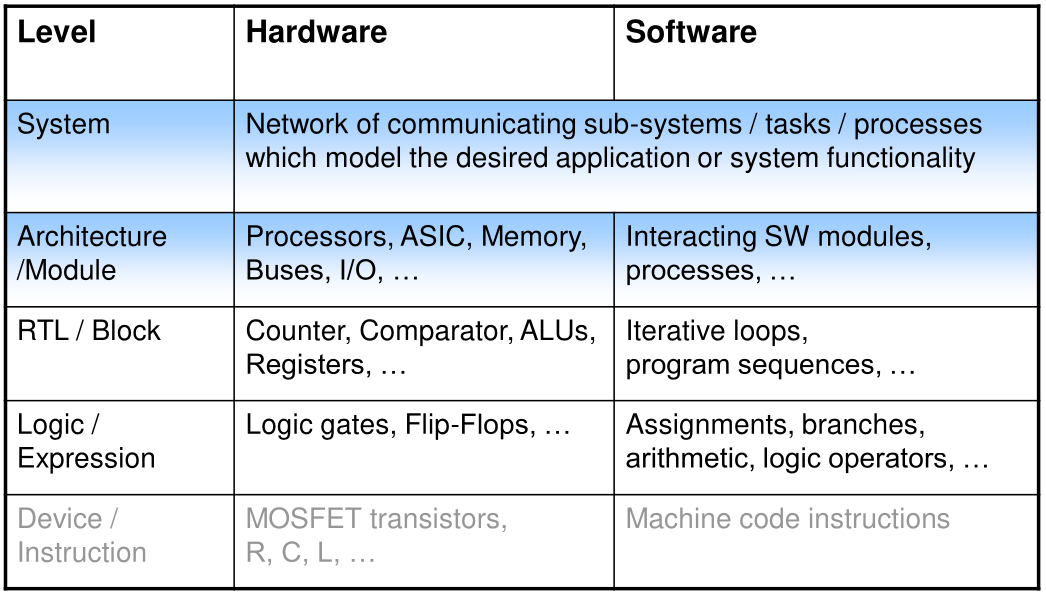
\includegraphics[width=0.8\linewidth]{assets/AbstractionLevels.png}
\end{center}


\section{Methodology}

\textbf{System Design} is the process to implement a desired function with a given set of physical or software components.

\textbf{Design Flow}: Sequence of individual steps of the design process

\textbf{Top-Down Design}
\begin{enumerate}
		\item \textbf{Specification} of the functional behavior
		\item \textbf{Exploration} of alternative realizations within the design space
		\item \textbf{Refinement} of the most promising realization towards the next lower abstraction level
\end{enumerate}

\paragraph{Specification, Exploration, Refinement}

\begin{center}
  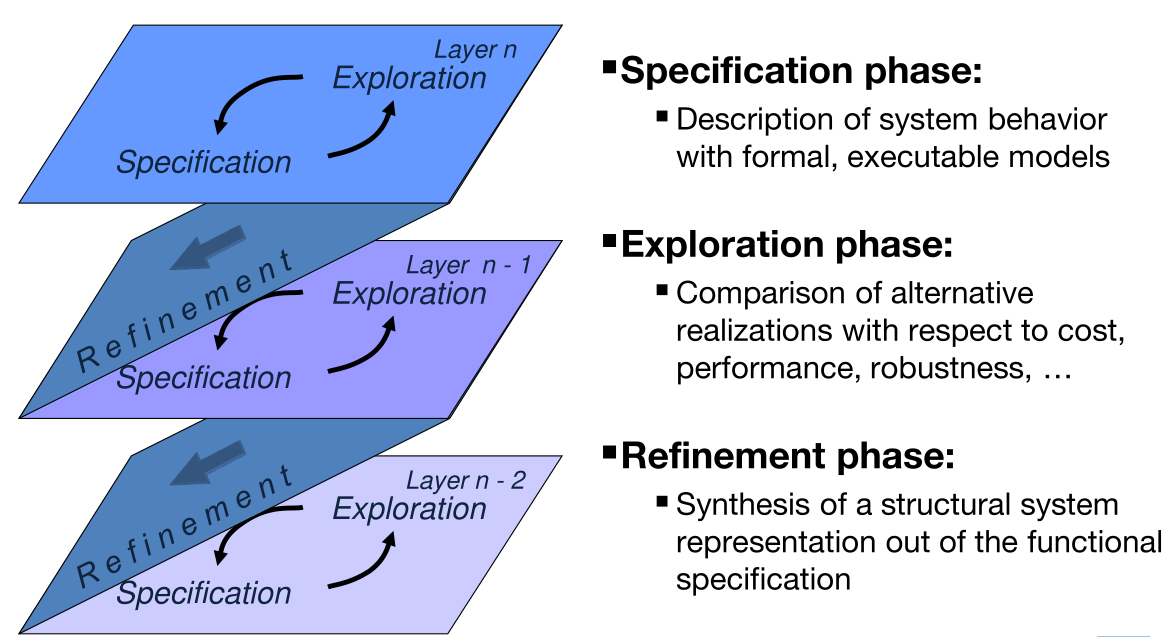
\includegraphics[width=0.8\linewidth]{assets/SpecExRef.png}
\end{center}

\textbf{Abstraction} Design flaws or errors resulting from imprecise modeling or insufficient exploration require abstraction and reiteration of design flow at next higher layer

Abstraction is possible in a top-down design strategy because it involves starting with a high-level, abstract view of the system and progressively refining it into detailed components.
 
\paragraph{Bottom Up Design}

\begin{center}
  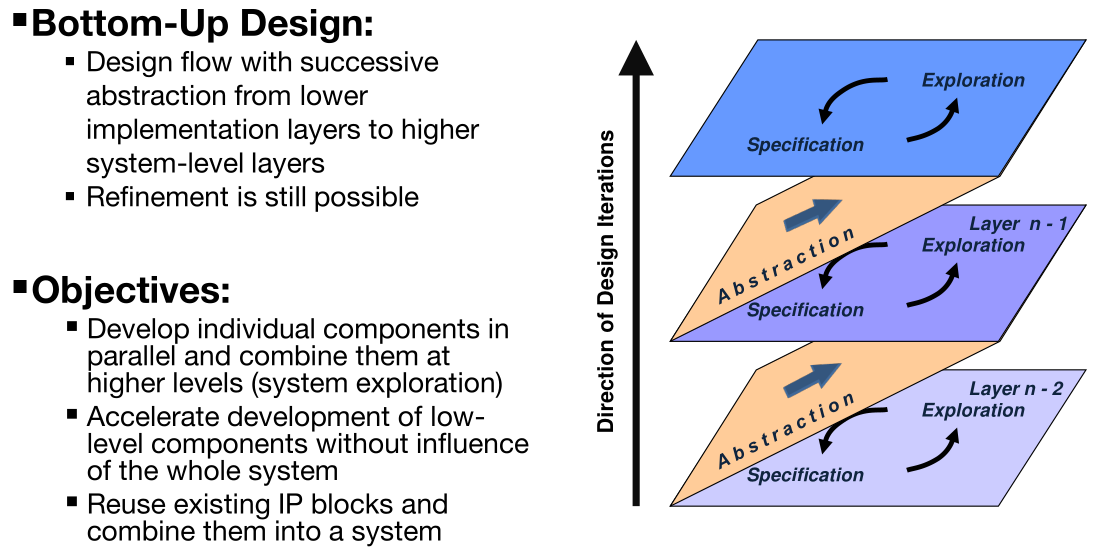
\includegraphics[width=0.8\linewidth]{assets/BottomUpDesign.png}
\end{center}
 
\paragraph{Meet in the Middle Strategy}

\begin{center}
  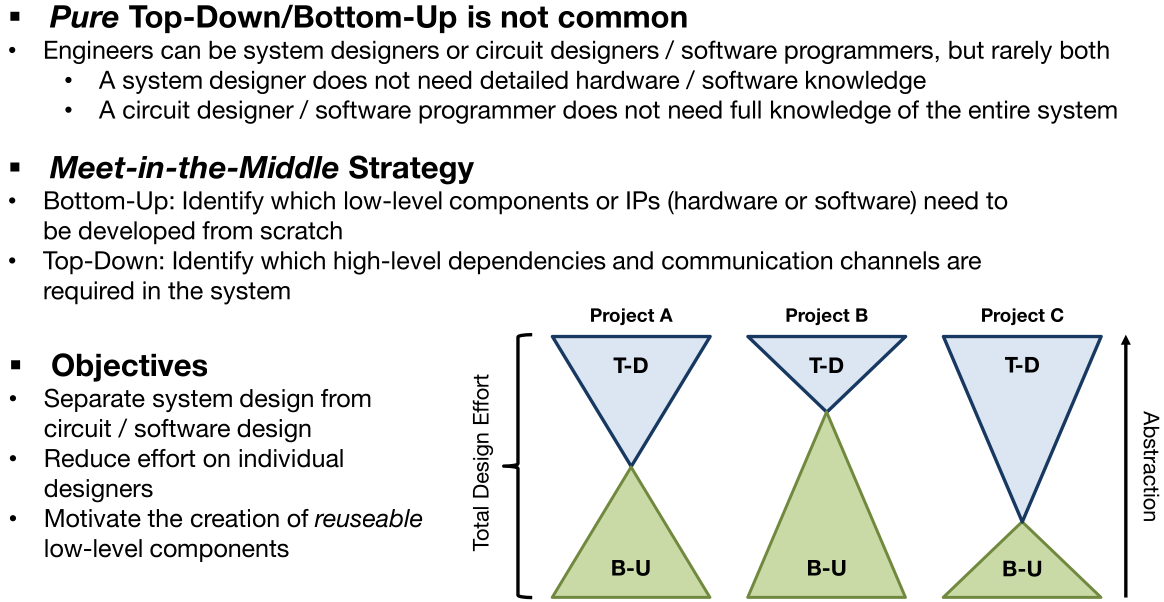
\includegraphics[width=0.8\linewidth]{assets/MeetInTheMiddle.png}
\end{center}

\paragraph{Simulation: Accuracy / Time Effort}

\begin{center}
  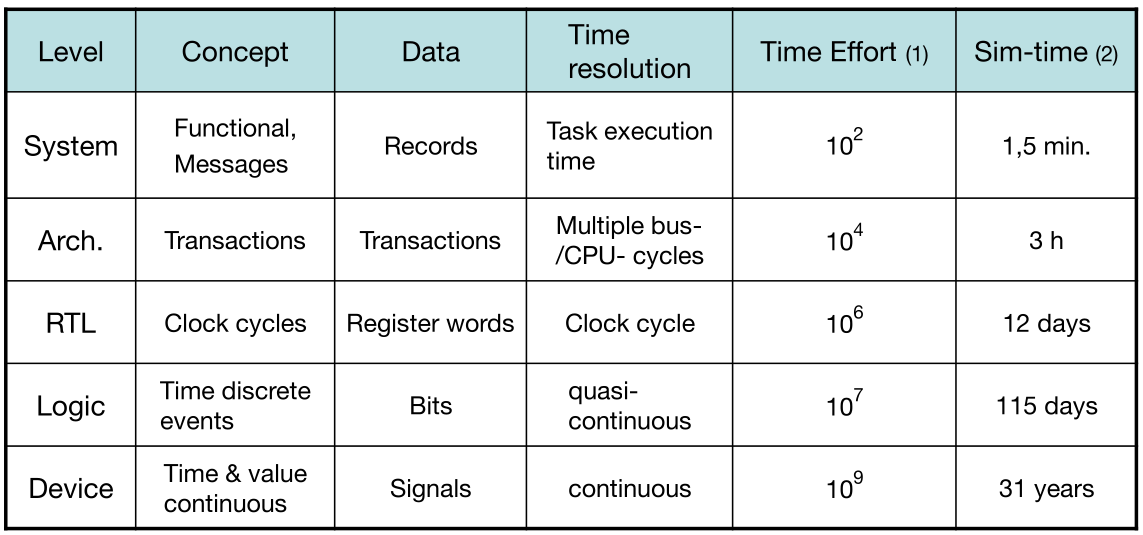
\includegraphics[width=0.8\linewidth]{assets/SimulationAccuracyTime.png}
\end{center}
 
\paragraph{Simualtion Acceleration}
\begin{enumerate}
	\item Divide and Conquer: parallel simulation - !validation of non parralelizable processes
	\item Mixed-Level Simulation - Some components simulation less accurate
	\item Reduction of Simulation Coverage - !Corner cases missed
\end{enumerate}
 
\paragraph{Design Views}

\begin{center}
  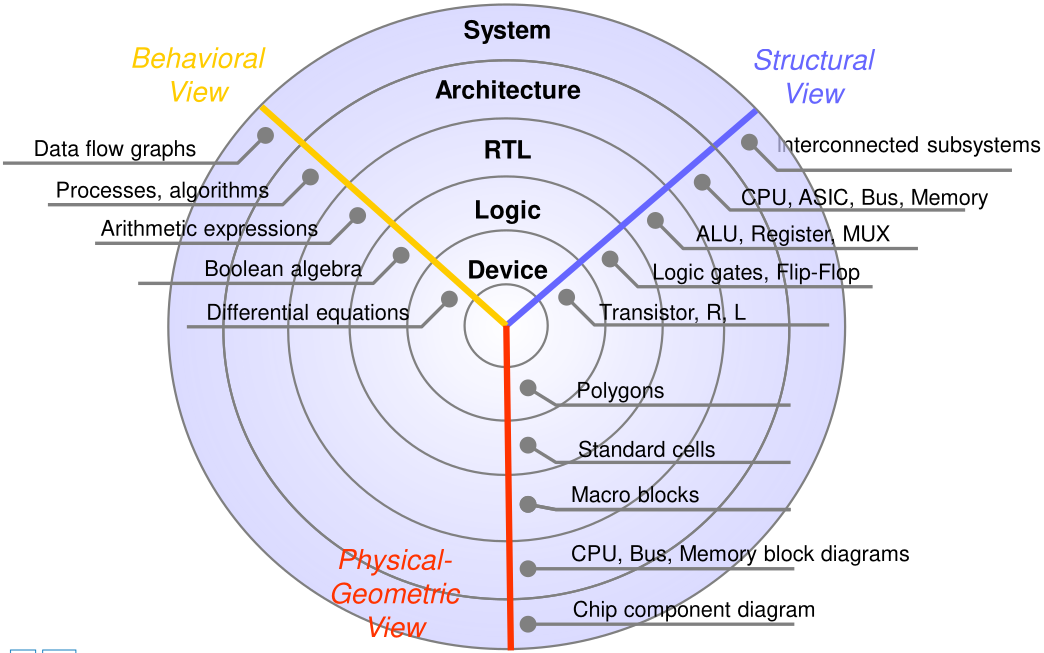
\includegraphics[width=0.8\linewidth]{assets/DesignViews.png}
\end{center}

\paragraph{DesignViewTransition}
\begin{center}
  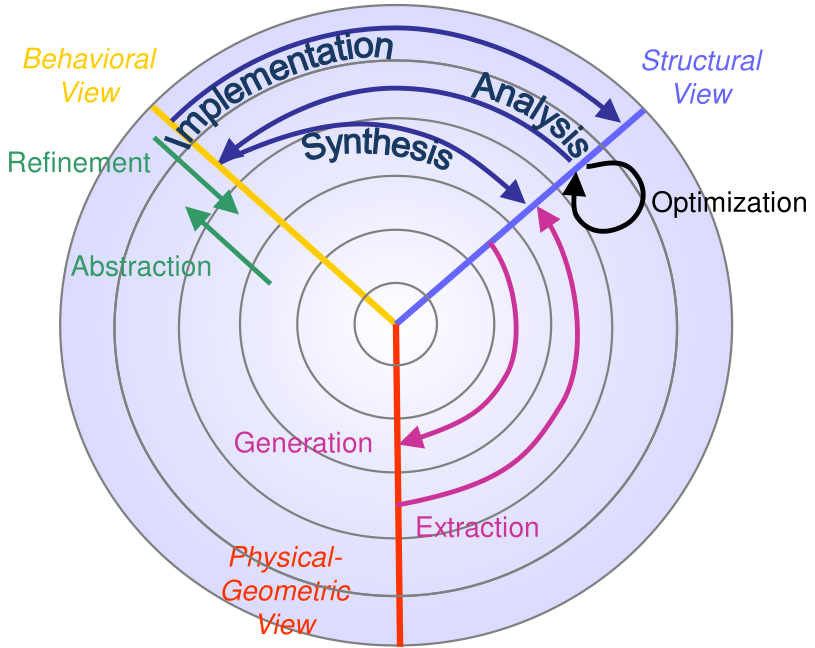
\includegraphics[width=0.7\linewidth]{assets/DesignViewTransitions.png}
\end{center}

\begin{center}
  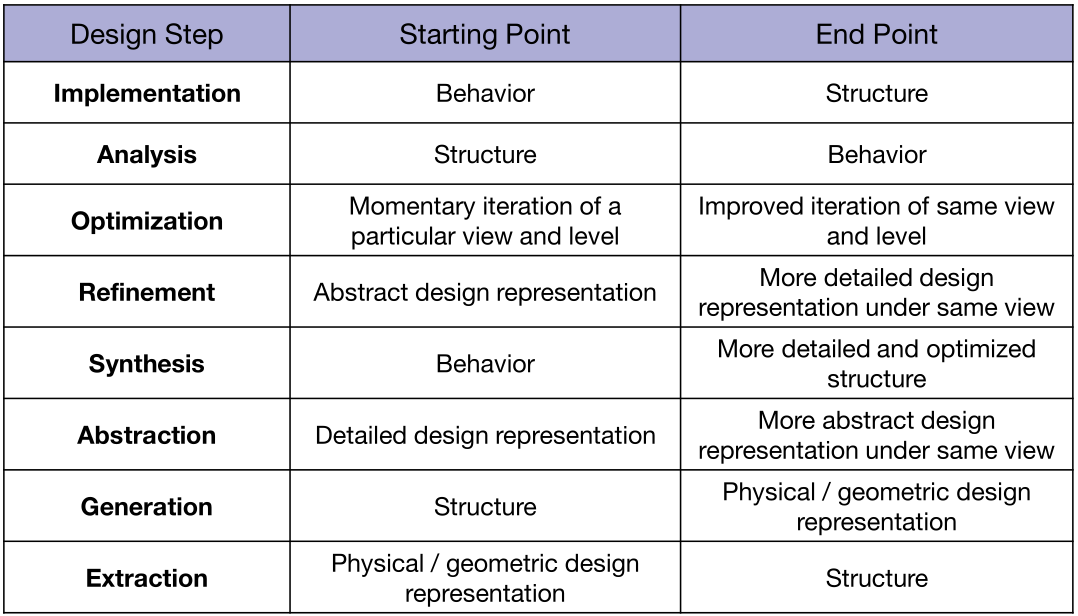
\includegraphics[width=0.8\linewidth]{assets/DesignViewTransitionTable.png}
\end{center}

\begin{center}
  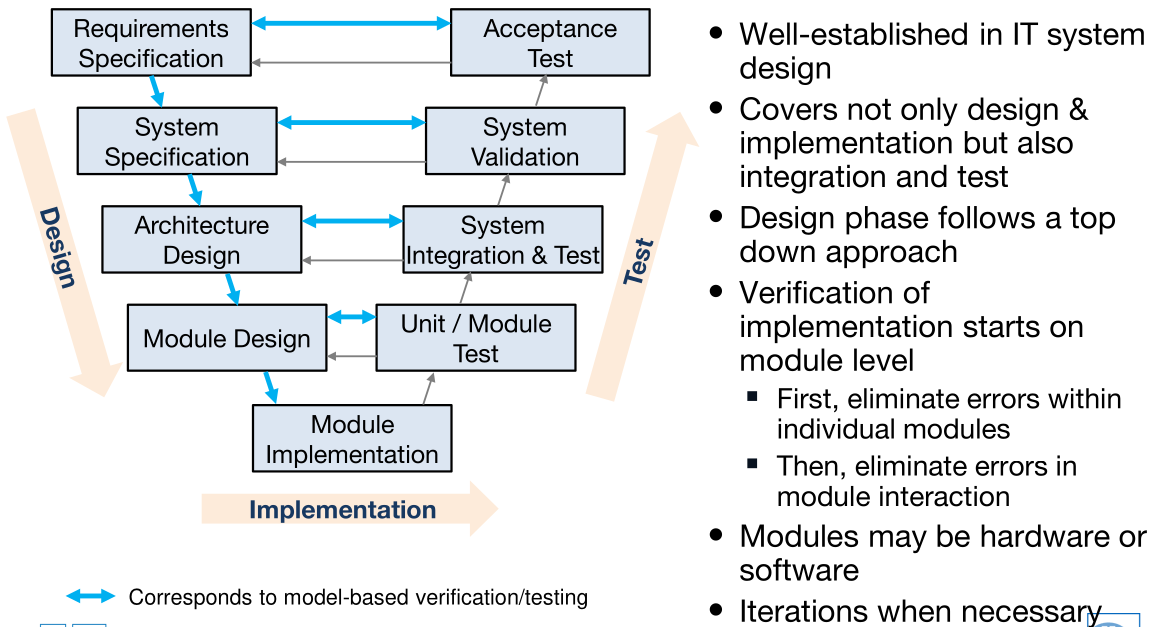
\includegraphics[width=0.8\linewidth]{assets/VModel.png}
\end{center}

\paragraph{Tutorial}

\textbf{linear extrapolation} $\frac{y - y_0}{x - x_0} = \frac{y_1 - y_0}{x_1 - x_0}$

\textbf{finite sum of positive integers} $\sum_{i=1}^{N} = \frac{N(N+1)}{2}$

\textbf{Difference from Solution} $\frac{after - before}{before}$
 
\textbf{Linear Time Complexity} $ O(N)$

\textbf{Quadratic Time Complexity} $ O(N^2)$

\textbf{Linearithmic Time Complexity} $ O(N log_2(N))$

\textbf{Execution Time} $T_{exec} = \frac{CPI \cdot Ops}{f_{cpu}}$
 
\textbf{Optimization} Parallelize tasks that are non dependent, run bottleneck tasks on HW


\section{Specification \& Modeling}

\begin{center}
  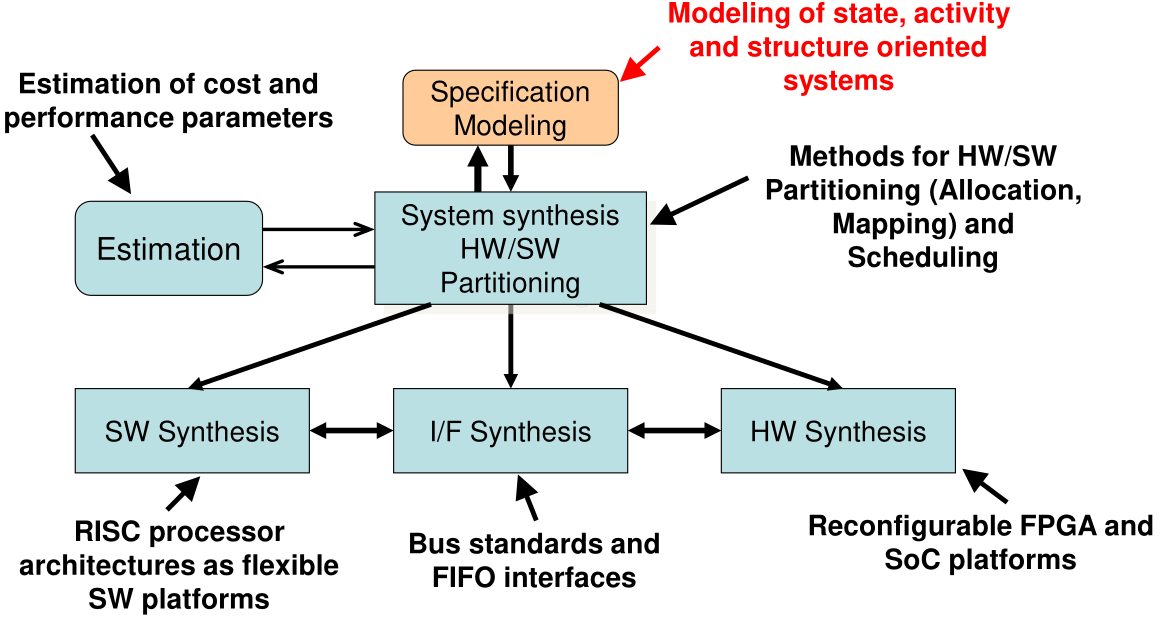
\includegraphics[width=0.8\linewidth]{assets/DesignFlowSystemLevel.png}
\end{center}

\textbf{system specification} defines
\begin{enumerate}
	\item functionality of the system
	\item constrains / properties (latency, power dissipation...)
\end{enumerate}

\textbf{Virtual Prototoypes} Alllow for HW and SW components of a system to be developed in parallel.

\paragraph{Models of Computation}

\begin{center}
  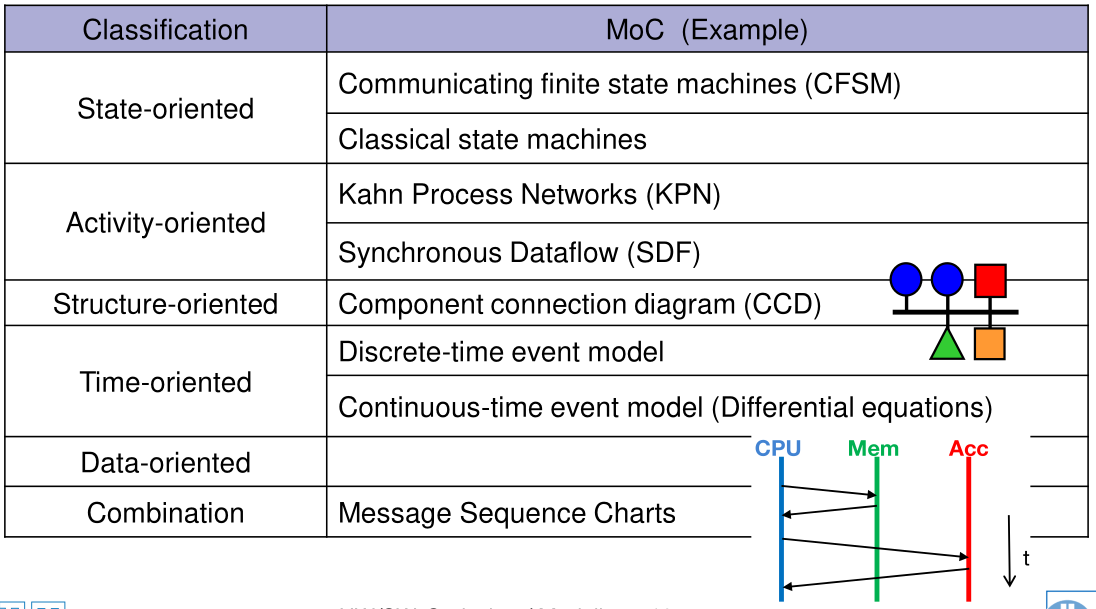
\includegraphics[width=0.8\linewidth]{assets/ModelsOfComputation.png}
\end{center}

\subsection{State-Oriented Models}

\paragraph{Finite State Machine}

\begin{center}[h]
  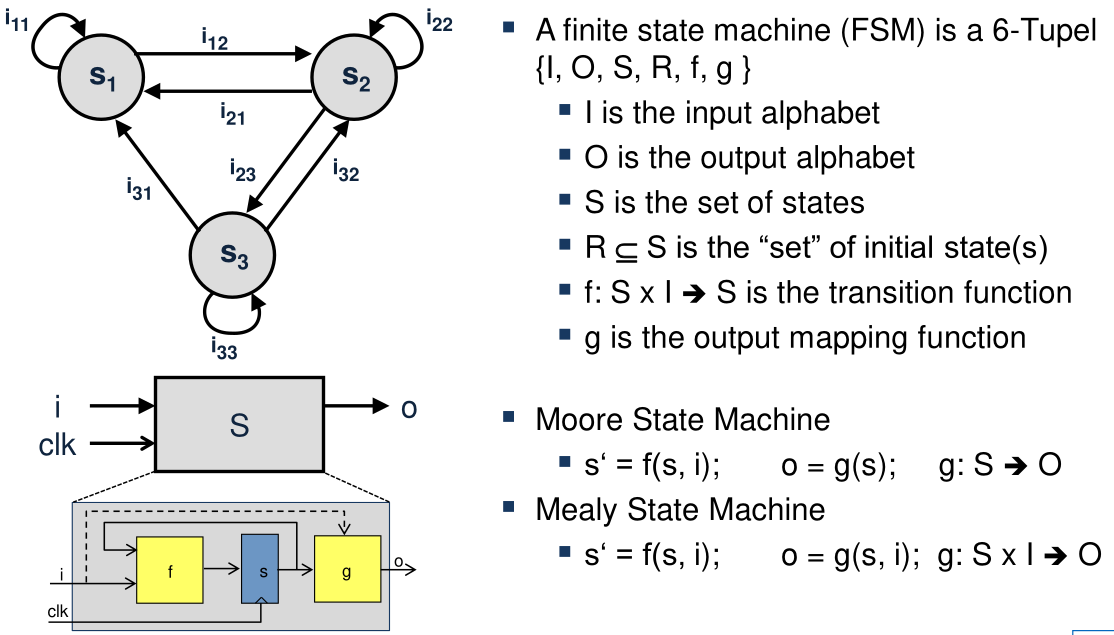
\includegraphics[width=0.8\linewidth]{assets/FiniteStateMachine.png}
  \label{fig:finitestatemachine}
\end{center}


\begin{center}
  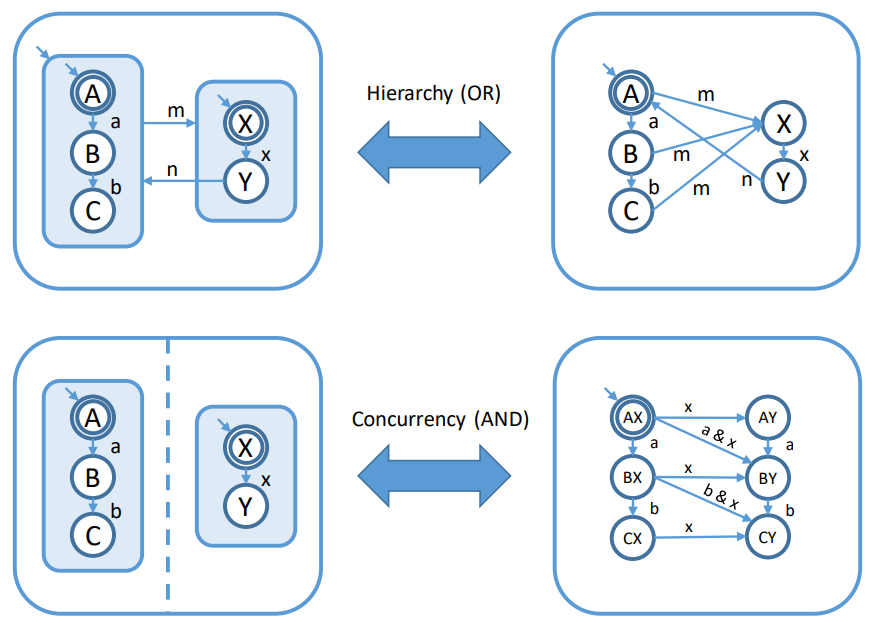
\includegraphics[width=0.8\linewidth]{assets/FSMTut.png}
  \label{fig:fsmtut}
\end{center}

\textit{Concurrency} is captured either by running multiple FSMs in parallel or by merging them into one large FSM whose states represent the combination of each sub-FSM’s states.

\textit{Synchronization} is captured through shared events, shared variables, or guard conditions that coordinate transitions among these concurrent machines.

\paragraph{Control Flow Graph}

\begin{center}
  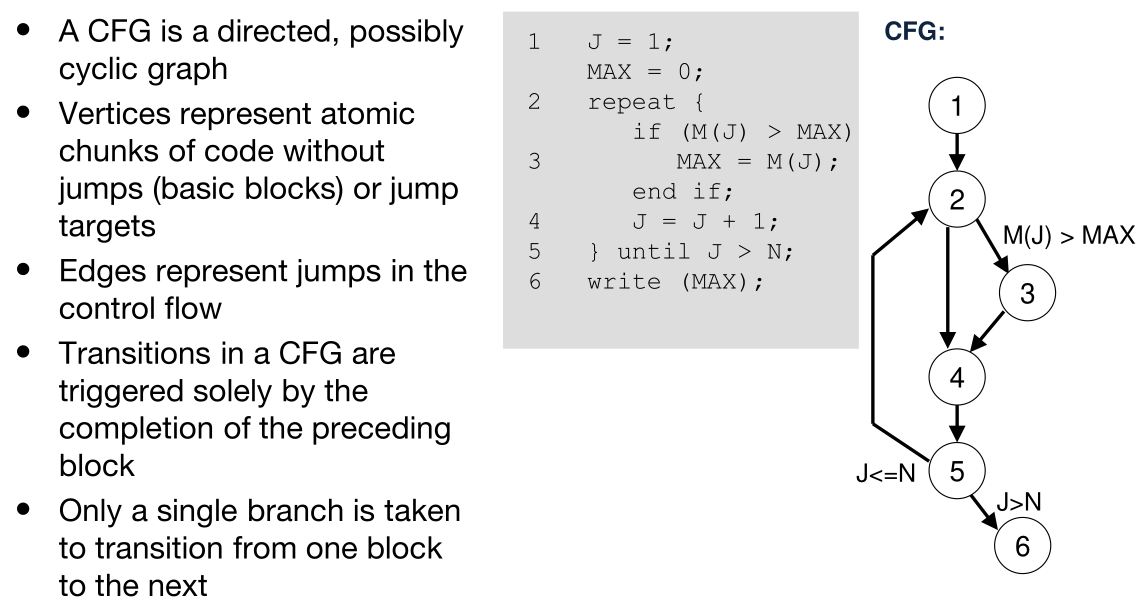
\includegraphics[width=0.8\linewidth]{assets/ControlFlowGraph.png}
  \label{fig:controlflowgraph}
\end{center}

\subsection{Activity Oriented Model}

\paragraph{Data Flow Graph}
 
\begin{center}
  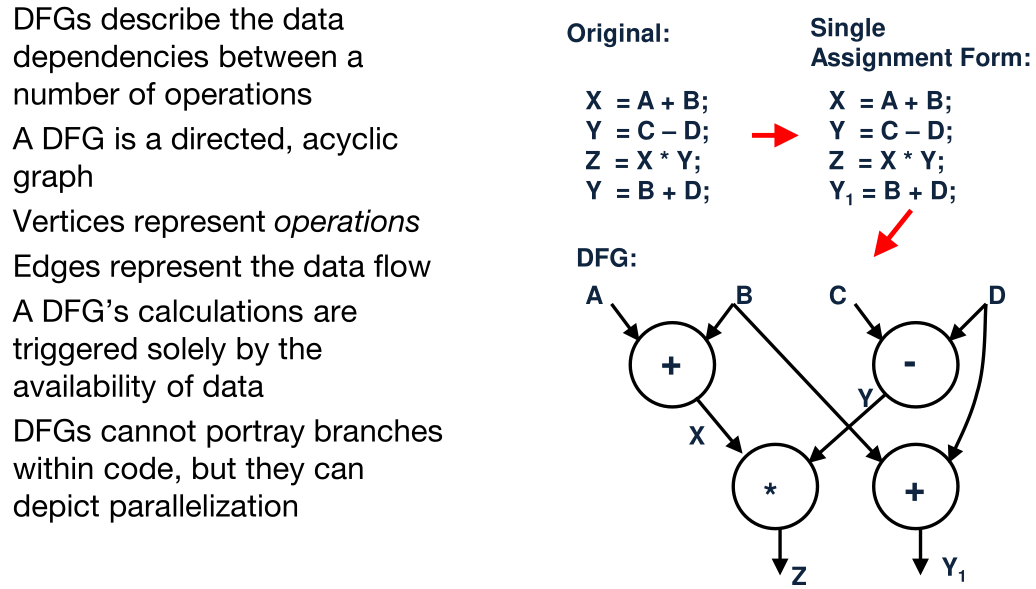
\includegraphics[width=0.8\linewidth]{assets/DataFlowGraph.png}
  \label{fig:dataflowgraph}
\end{center}

\paragraph{Kahn Process Networks (KPNs)}

\textbf{deadlocks}
\begin{enumerate}
  \item \textbf{True deadlock}: read from an empty buffer (KPN read semantics) which is never filled again
\item \textbf{Artificial deadlock}: write into a full buffer (bounded memories) which is never read again
\end{enumerate}

\textbf{Boundness}: Does the schedule require infinite memory?

\textbf{Completeness}: Do all processes get to run indefinitely?

\textbf{Non-Termination}: Will the there be deadlocks?

\textbf{Data driven scheduling}
\begin{enumerate}
	\item execute a process as soon as tokens are available
	\item Does not necessarily find a schedule with bounded buffers even if one exists
	\item Prefers completeness over boundedness
\end{enumerate}

\begin{center}
  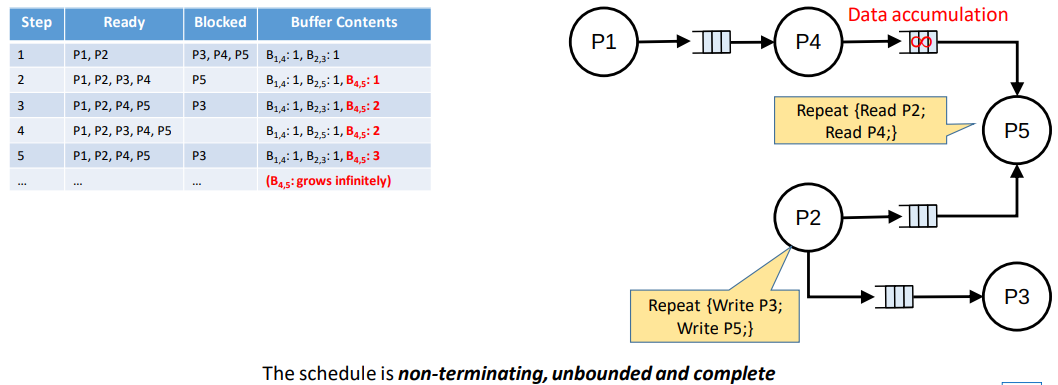
\includegraphics[width=0.8\linewidth]{assets/KPNDataExample.png}
  \label{fig:kpndataexample}
\end{center}

\textbf{Parks' Algorithm}: finds a schedule with bounded buffers if one exists
\begin{enumerate}
	\item Start with buffer size 1 for all channels.
	\item Apply data driven schedule.
	\item If termination occurs, increase buffer sizes by 1.
	\item Repeat.
	\item[$\bullet$] Prefers boundedness over completeness (non-termination)
	\item[$\bullet$] It is not guaranteed that Parks’ Algorithm finds a bounded and complete schedule
\end{enumerate}

\begin{center}
  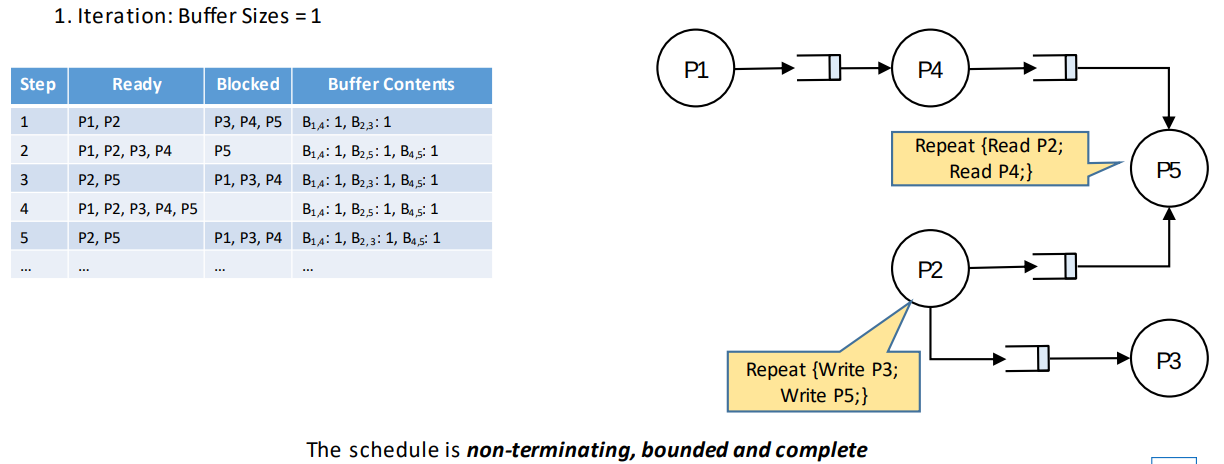
\includegraphics[width=0.8\linewidth]{assets/KPNExamplePark.png}
  \label{fig:kpnexamplepark}
\end{center}
 
\textbf{Properties KPN} No matter what the execution speed or schedule of the processes is, the KPN will always give the same result -$>$ Independent of timing -$>$ deterministic

\subsection{Synchronous Dataflow (SDF)}
SDF models can be used to define bounded schedules of execution. The maximum amount of
tokens needed to be held in a single communication channel can be determined through the
schedule.

\begin{center}
  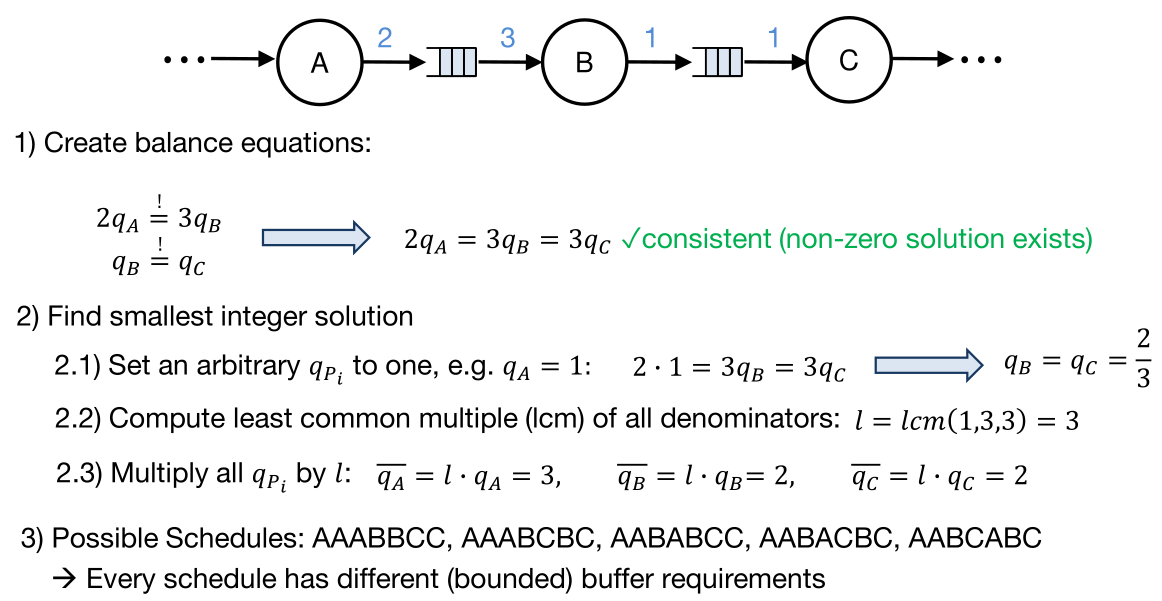
\includegraphics[width=\linewidth]{assets/SDFExample.png}
  \label{fig:sdfexample}
\end{center}
 
\begin{center}
  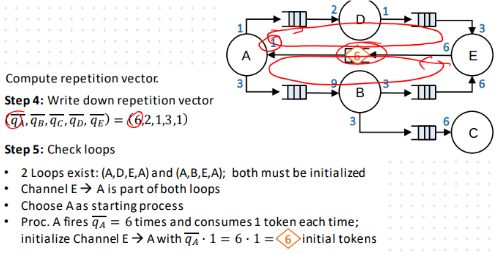
\includegraphics[width=\linewidth]{assets/SDFExample2.png}
  \label{fig:sdfexample2}
\end{center}

\paragraph{Structure Oriented Model}

\paragraph{Data Oriented Model}

\paragraph{Concurrency}
It is often simpler and more concise to portray the behavior of a system as a set of multiple concurrent sub-behaviors

Concurrency generally refers to the ability of a system to handle multiple tasks (or parts of tasks) at overlapping time periods, rather than doing them strictly one after another.

\paragraph{Hierarchy}

\paragraph{Structural-/Behavioral-Hierarchy}

\paragraph{Program Structures/Constructs}

\paragraph{Completion}

\paragraph{Communication}
\begin{enumerate}
  \item Shared-memory communication
    \begin{enumerate}
      \item The sending process writes a global variable into a shared resource (shared memory)
      \item All receiving processes can now read this variable (good broadcasting properties)
      \item Any necessary synchronization must be accomplished separately
    \end{enumerate}
  \item Message passing communication
    \begin{enumerate}
    	\item Data is exchanged between processes using a communication channel to pass messages
	\item Processes can access the channel using send/receive primitives
	\item At higher levels of abstraction, channels are virtual entities and not bound by implementation details
	\item  Channels can be unidirectional or bidirectional, using a point to point or shared (addressed) bus infrastructure
    \end{enumerate}

    \textbf{Blocking transfer} the sending process waits until the receiving process has accepted (or is ready to provide) the data (requires synchronization of the processes prior to the transfer, and can have potential deadlocks)

    \textbf{non-blocking transfer} the sending process writes the data into a queue and immediately continues processing. The receiving process can then read the data from the queue at its leisure. This allows the sending and receivingprocesses to work independently, but requires additional memory (queues). (unbounded)
\end{enumerate}

\paragraph{Synchronization}
\begin{enumerate}
  \item Control-oriented synchronization
    \begin{enumerate}
    	\item The control structure of the behavioral description determines the synchronization between processes
    \end{enumerate}
  \item Data-oriented synchronization
    \begin{enumerate}
    	\item Synchronization is accomplished using inter-process communication
	  \begin{enumerate}
	    \item Synchronization using shared memory
	    \item Synchronization using message passing
	  \end{enumerate}
    \end{enumerate}
\end{enumerate}
 
\paragraph{Exception Handling} Certain events, such as a reset or CPU interrupt, can necessitate the abrupt termination of a process

\paragraph{Non-Determinism} Occasionally it may be unclear which of several state transitions or
sequences of operations are best suited for the application at hand

\section{Synthesis}

\paragraph{Design Synthesis} 
Combined process of Implementation, Refinement(and Optimization)

\textbf{Central tasks of design synthesis:}

\begin{enumerate}
	\item Allocation: Selection and provisioning of processing resources
	\item Mapping: Assignment of functions to resources
	\item Scheduling: Determination of execution sequences and start times for tasks/processes under consideration of data dependencies in the task graph
\end{enumerate}

\paragraph{System Synthesis}
\begin{enumerate}
  \item Allocation: Determine
    \begin{enumerate}
      \item type and number of CPU/DSP cores,
      \item size of memories,
      \item standard and application specific hardware building blocks,
      \item  I/O interfaces and
      \item interconnect structures
    \end{enumerate}
  \item Mapping: Assignment of entire sub-systems / tasks of the system model to HW / SW resources (HW/SW-Codesign)
    \begin{enumerate}
      \item Scheduling: Determine the
      \item execution sequence of tasks and communication transactions between different resources
      \item execution sequence of tasks which have been mapped to the same resource
    \end{enumerate}
\end{enumerate}

\paragraph{Task Graph}

\begin{center}
  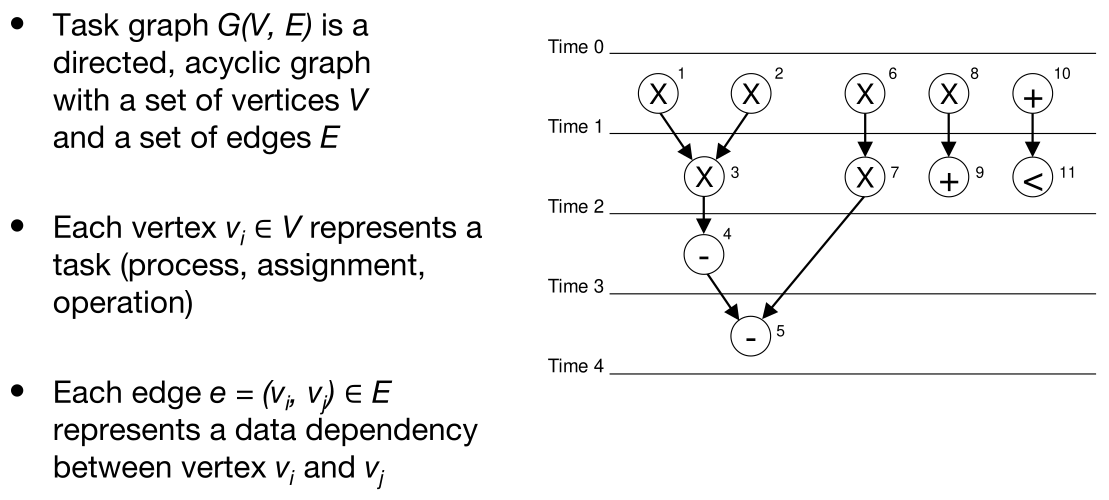
\includegraphics[width=\linewidth]{assets/TaskGraph.png}
  \label{fig:taskgraph}
\end{center}

\paragraph{Resource Graph}

\begin{center}
  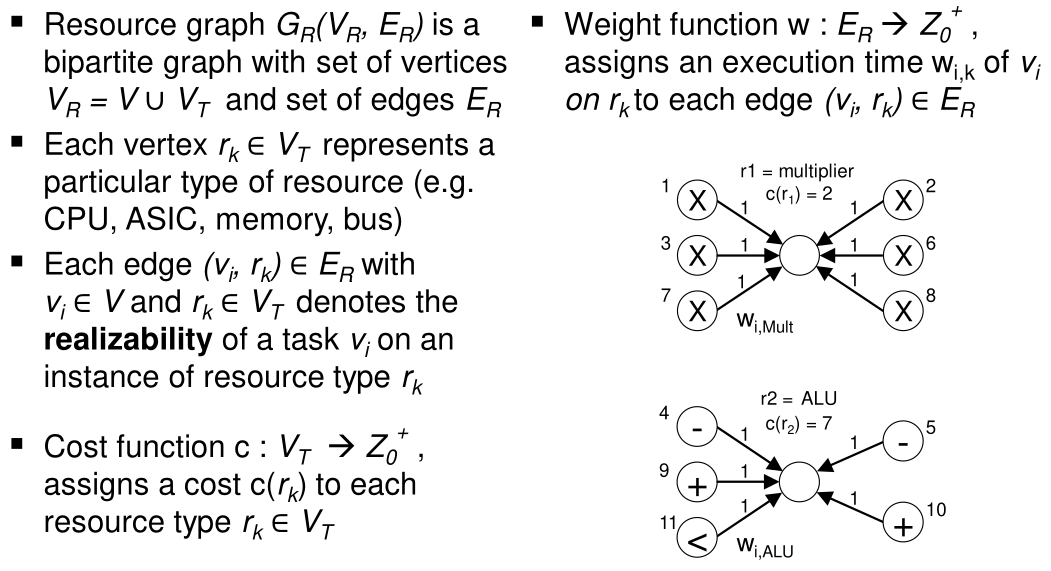
\includegraphics[width=\linewidth]{assets/ResourceGraph.png}
  \label{fig:resourcegraph}
\end{center}

\paragraph{Architecture Graph}

\paragraph{Allocation} Allocation is a function $\alpha$ ..

\paragraph{Mapping}

\paragraph{Partitioning Problem}

\begin{center}
  \centering
  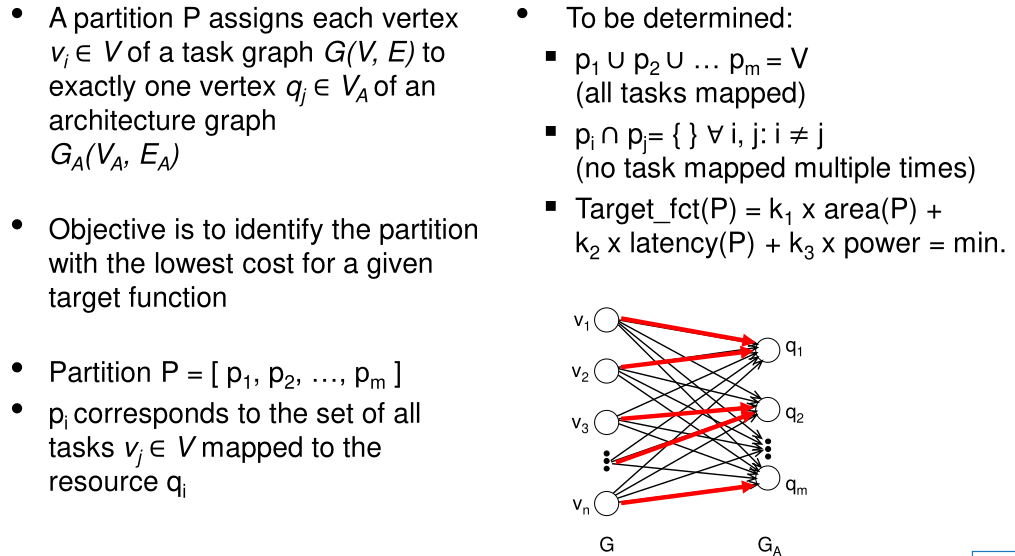
\includegraphics[width=\linewidth]{assets/PartitioningProblem.png}
  \label{fig:partitioningproblem}
\end{center}

\textbf{Complexity of partitioning problem}
\begin{enumerate}
	\item m: architecture components
	\item n: task objects
	\item $O(m^n)$
	\item $nPartitions = \prod_i m_i^{n_i}$
\end{enumerate}

\paragraph{Schedule}

\begin{center}[h]
  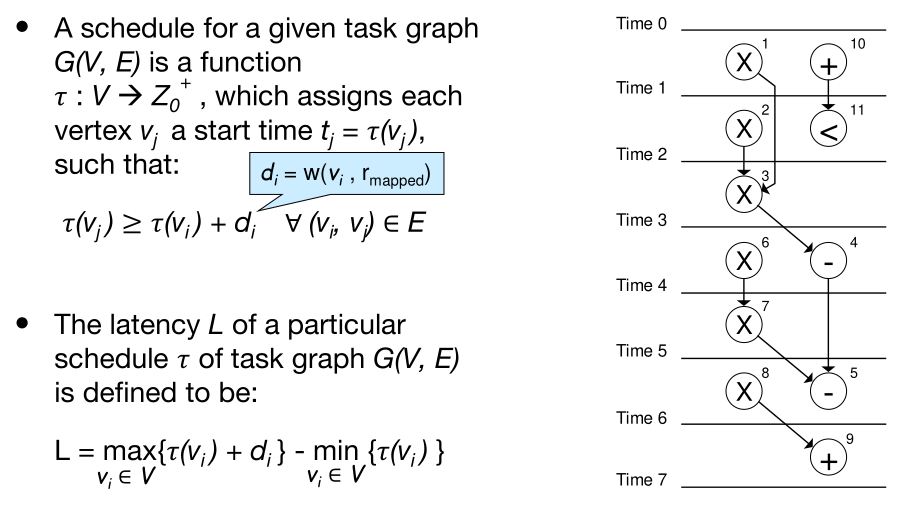
\includegraphics[width=\linewidth]{assets/Schedule.png}
  \label{fig:schedule}
\end{center}

\paragraph{Design Space Exploration}

\paragraph{Pareto Analysis}
% \begin{center}
%   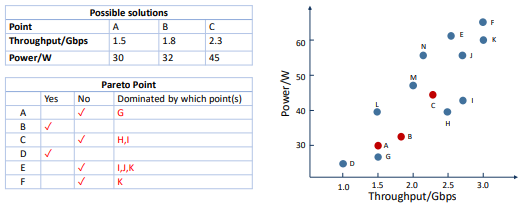
\includegraphics[width=0.8\linewidth]{assets/ParetoTutorial.png}
%   \label{fig:paretotutorial}
% \end{center}

\begin{center}
  \centering
  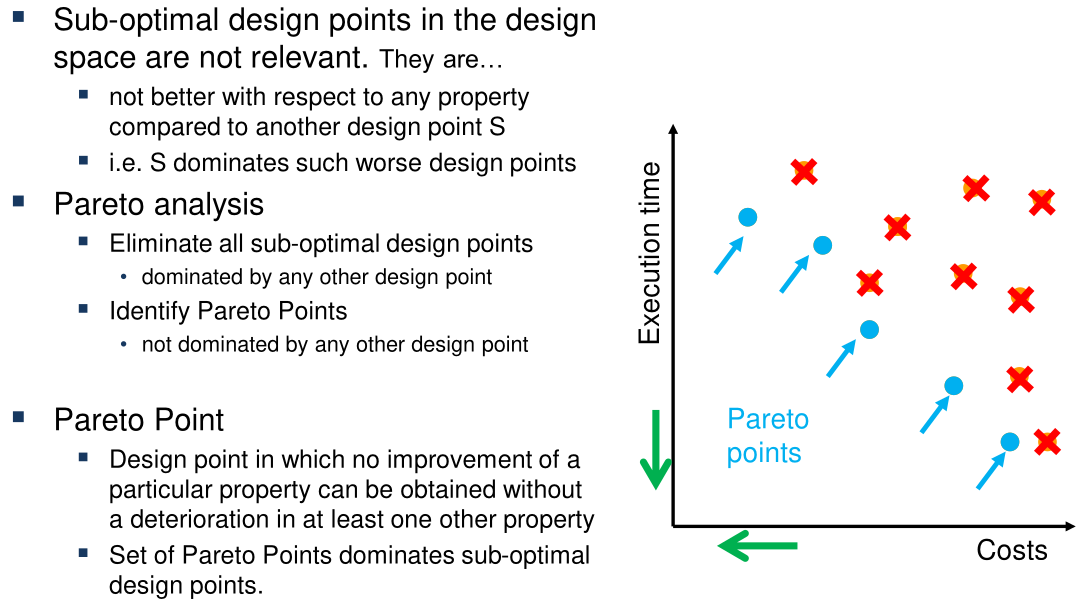
\includegraphics[width=\linewidth]{assets/ParetoSlide.png}
  \label{fig:paretoslide}
\end{center}

\paragraph{Partitioning Methods}

\paragraph{ILP}

\paragraph{Heuristic Methods}
A technique designed for solving a problem more quickly when classic methods are too slow, or for finding an approximate solution when classic methods fail to find any exact solution. This is achieved by trading optimality, completeness, or precision for speed.

\textbf{Closeness}: Measure derived from multiple metrics indicating a force to group two functional objects during a partitioning process

\paragraph{Constructive Methods}
\begin{enumerate}
  \item Random grouping
    \begin{enumerate}
      \item Tasks are randomly mapped to resources in sequential fashion
      \item  Indepent of closeness values
      \item Method of complexity O(n)
    \end{enumerate}

  \item Hierarchical Clustering
    \begin{enumerate}
      \item (Functional) object / task is assigned to a group
      \item Closeness is criterion for assignment
      \item Subsequent recalculation of closeness functions
      \item Iteration of above steps till termination condition is fulfilled
    \end{enumerate}
\end{enumerate}

\paragraph{Hierarchical Clustering}

\begin{center}
  \centering
  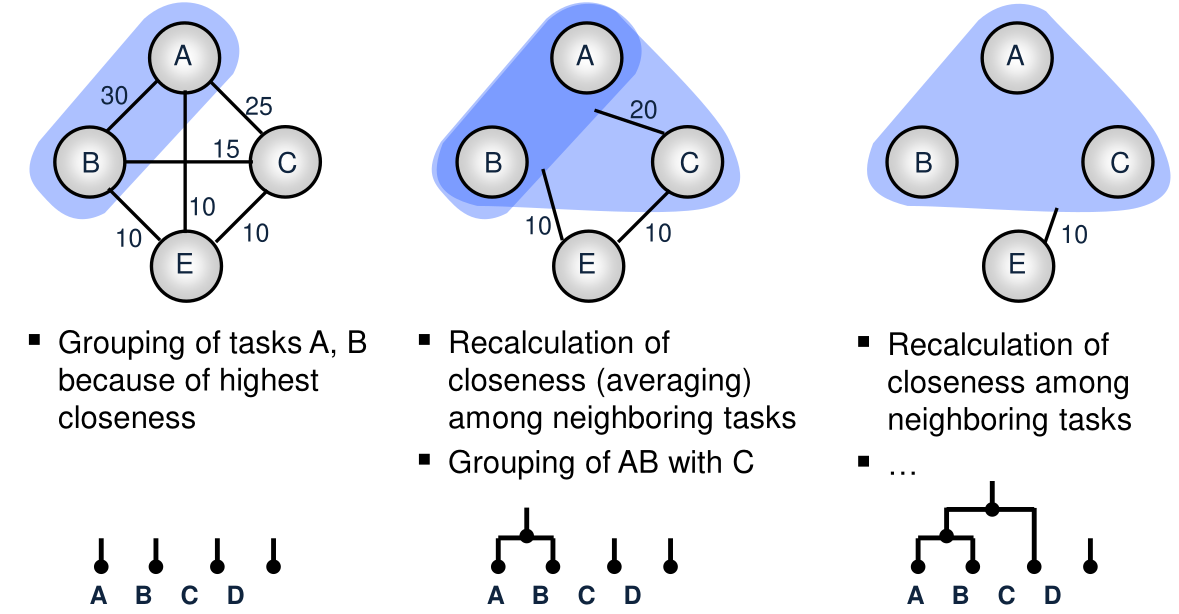
\includegraphics[width=0.8\linewidth]{assets/HierarchicalClustering.png}
  \label{fig:hierarchicalclustering}
\end{center}

\textbf{Termination Criteria}
\begin{enumerate}
	\item Number of remaining clusters / groups
	\item Getting below a certain closeness boundary (e.g. $\leq$ 15)
\end{enumerate}

\textbf{Characteristics}
\begin{enumerate}
	\item $O(n^2)$: Still applicable to sets with large number of objects
	\item Based on concept of local optimization; cannot overcome local minima
	\item Frequently used to obtain an initial partition with subsequent iterative improvements
\end{enumerate}

\paragraph{Group Migration – Min Cut}
\begin{enumerate}
  \item Move individual objects to different groups and determine the resulting deltas in the target function
  \item Object with biggest reduction / smallest increase in target function is moved to new group
  \item Every object can be moved only once
  \item When all objects have been moved once, select partition with best target function
\end{enumerate}

$\Delta = connection_{samePartition} - connection_{newPartition}$ 

\textit{Watch out that all connections to same / other partition are considered!}

\begin{center}
  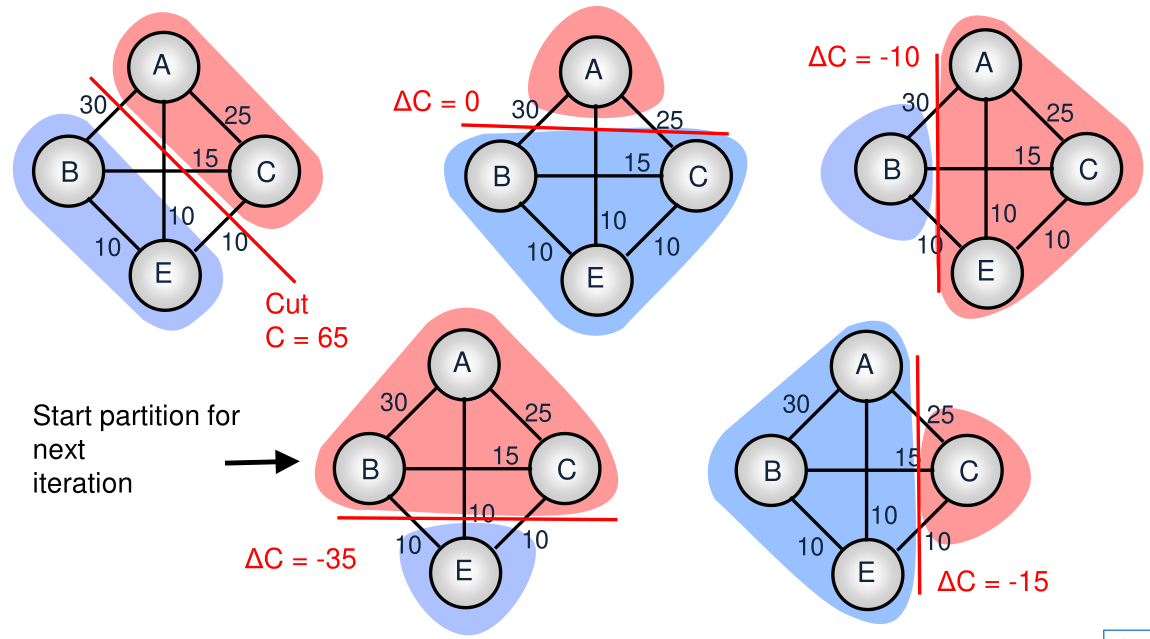
\includegraphics[width=0.8\linewidth]{assets/MinCut.png}
  \label{fig:mincut}
\end{center}

\textbf{Rate Cut method} Prevent clustering of all objects into a single group

$Ratio = \frac{cut(P)}{size(p_1) \cdot size(p_2)}$

\paragraph{Simulated Annealing}
\begin{enumerate}
	\item Idea is inspired by annealing process of melted mass
	\item Simulated degradation of temperature T such that a thermal equilibrium is attained for each T
	\item The bigger the cost delta and the runtime, the lower is the probability to accept an inferior partition
	\item optimal method when temperature degradation happens arbitrarily slowly
	\item Computational complexity of the method depends on actual implementation and can vary between exponential and polynomial
\end{enumerate}


Applied to partitioning problem
\begin{enumerate}
	\item  Method of statistical iterative improvement 
	\item Acceptance of inferior partitions depends on :
	  \begin{enumerate}
	  	\item The absolute cost delta
		\item The runtime of the method
	  \end{enumerate}
\end{enumerate}

\begin{center}
  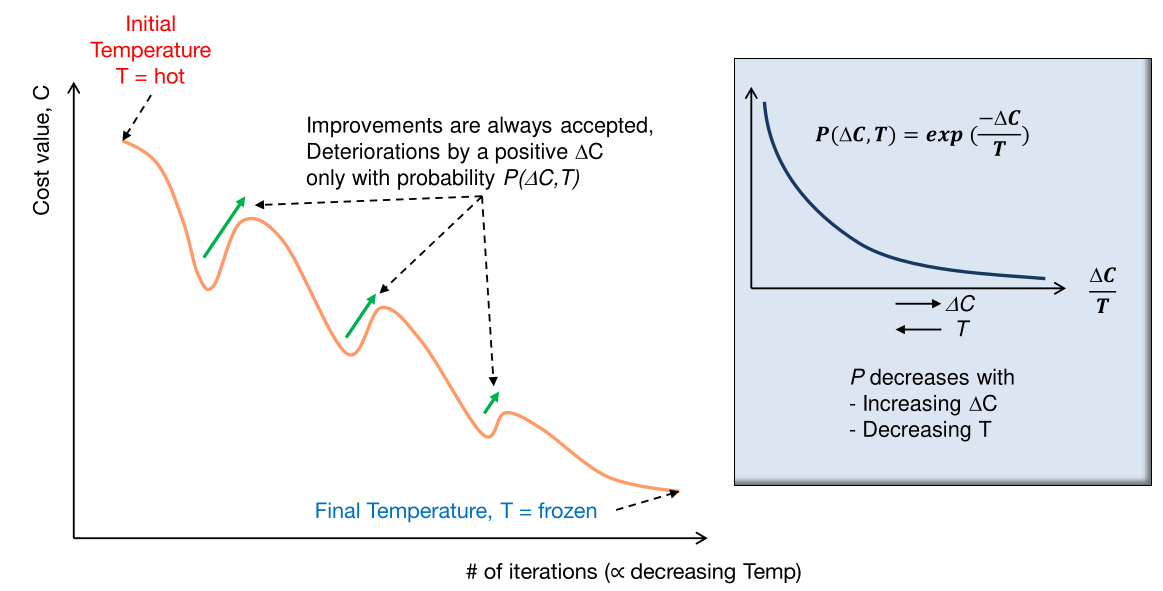
\includegraphics[width=0.8\linewidth]{assets/SimulatedAnnealing.png}
  \label{fig:simulatedannealing}
\end{center}

\paragraph{Greedy Partitioning}
Starting from a pure SW partition objects are moved into HW partition until performance requirements are met
$P_{init} = \{ p_{sw}, p_{hw} \} = \{ O, \O \}$

\paragraph{Grupta Partitioning}
Starting from a pure HW partition, objects are moved to SW partition as long as performance requirements are still met and target function is improved
$P_{init} = \{ p_{sw}, p_{hw} \} = \{ \O, O \}$

\paragraph{Tabu Search}

\begin{center}
  \centering
  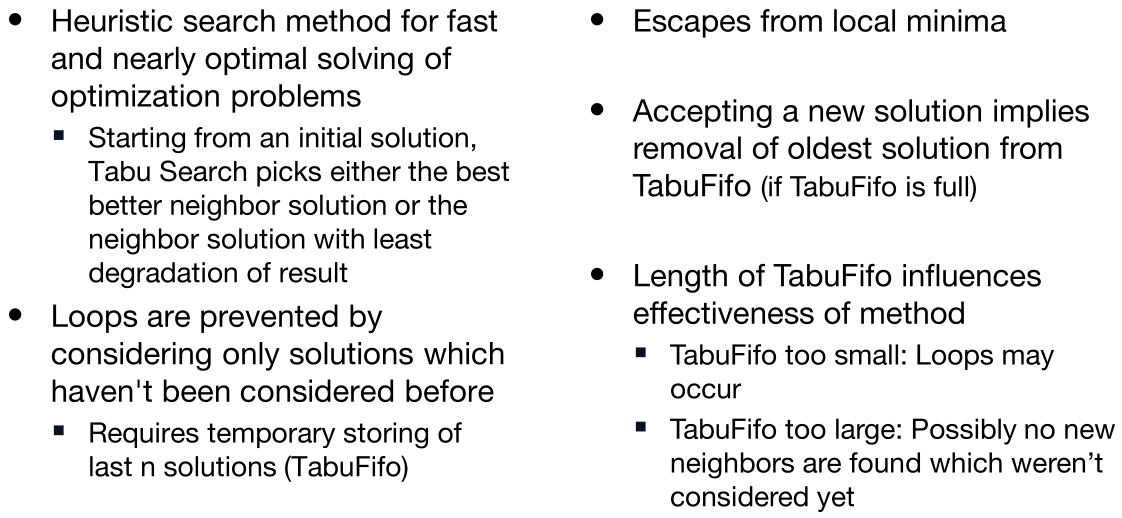
\includegraphics[width=\linewidth]{assets/TabuSearch.png}
  \label{fig:tabusearch}
\end{center}

\begin{center}
  \centering
  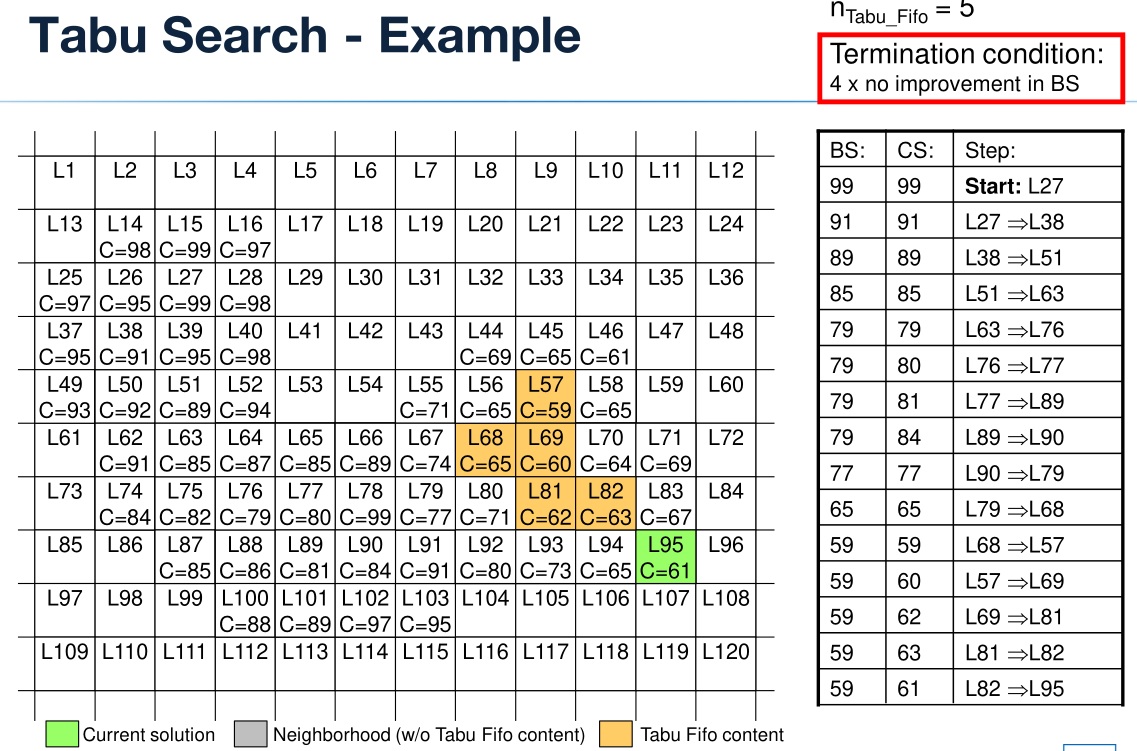
\includegraphics[width=\linewidth]{assets/TabuExample.png}
  \label{fig:tabuexample}
\end{center}

\paragraph{Genetic Algorithms}

\begin{center}
  \centering
  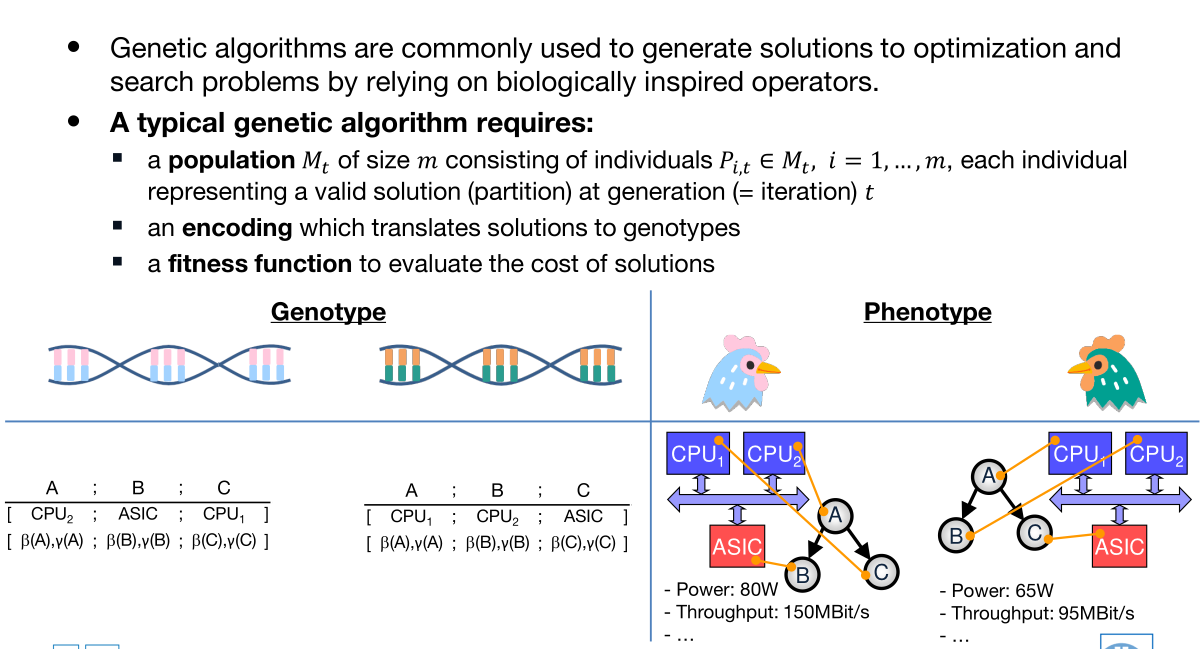
\includegraphics[width=\linewidth]{assets/GeneticAlgortihm.png}
  \label{fig:geneticalgortihm}
\end{center}

\begin{center}
  \centering
  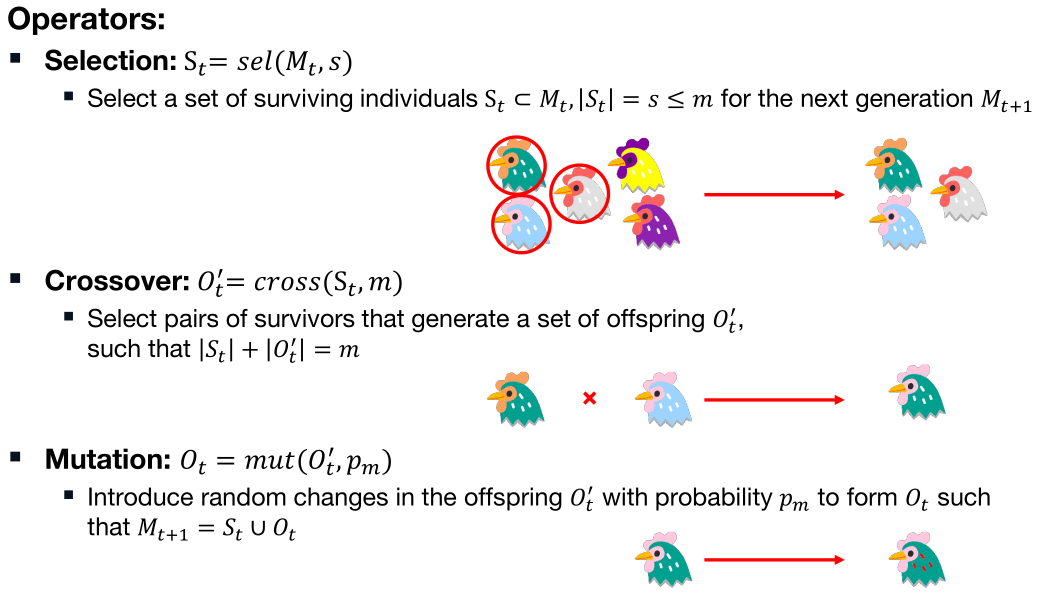
\includegraphics[width=0.8\linewidth]{assets/GeneticOperators.png}
  \label{fig:geneticoperators}
\end{center}

\begin{center}
  \centering
  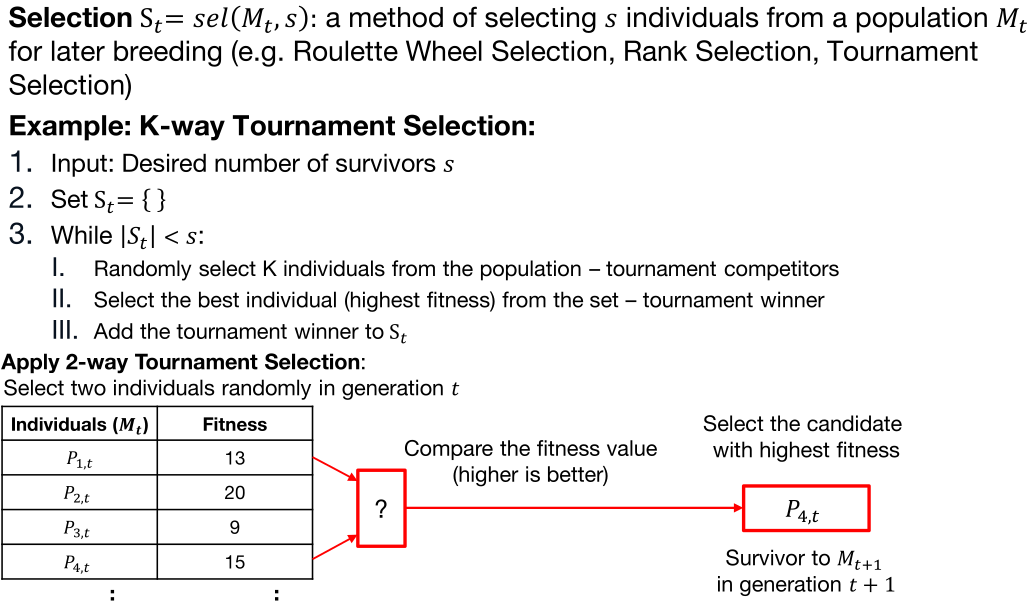
\includegraphics[width=0.8\linewidth]{assets/GeneticSelection.png}
  \label{fig:geneticselection}
\end{center}

\begin{center}
  \centering
  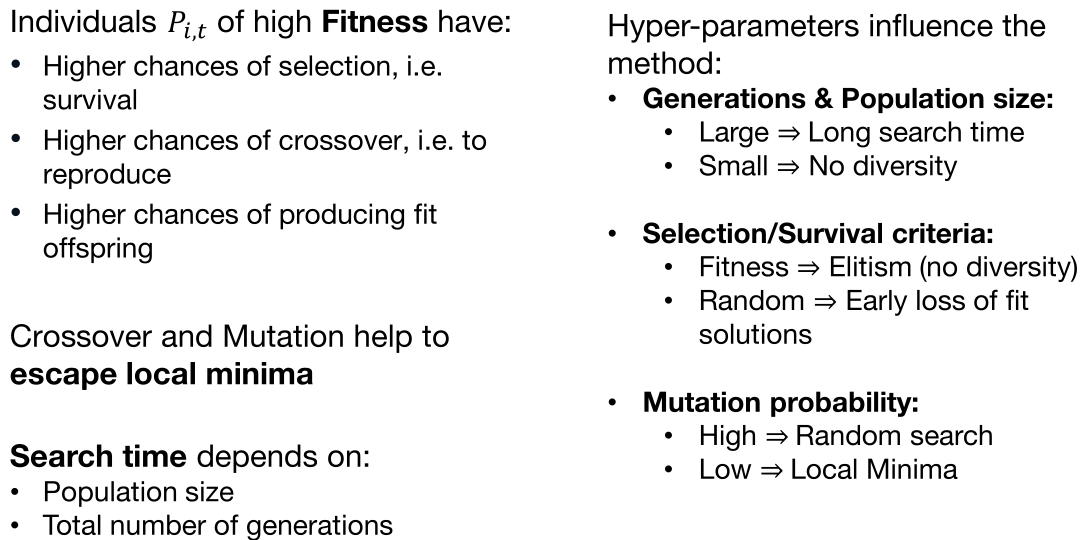
\includegraphics[width=0.8\linewidth]{assets/GeneticCharacteristics.png}
  \label{fig:geneticcharacteristics}
\end{center}

\section{Scheduling}
Determines the execution sequence and start times of tasks/jobs on processors under consideration of task priorities, task deadlines and data dependencies in the task/problem graph

\textbf{Static / off-line scheduling}: Determines the execution sequence and
start times of jobs at design or compilation time

\textbf{Scheduling without resource constrains}: (Theoretically) relevant to determine the lower bound of (processing)

\textbf{Preemptive scheduling}: Possibility to interrupt execution of a
task/process during run time (to the benefit of another task/process) and
resume execution on same or different resource

\textbf{Dynamic / on-Line scheduling}: Determines the execution sequence and
start times of jobs at run time

Dynamic methods are more flexible and may lead to better processor utilization. Correct system behavior of static methods are way easier to guarantee.

\textbf{Scheduling with resource constraints}: Consider availability of limited processing resources during scheduling

\textbf{Periodic scheduling}: Scheduling of iterative tasks / processes with execution interval (period) T, relative deadline $t_d$ and priority

\textbf{Sporatic sceduling}: Schedule sporatic occuring tasks with bounded rate and lower-bound inter arrival rate, but possibly assigned priority and deadline
latency


\begin{center}
  \centering
  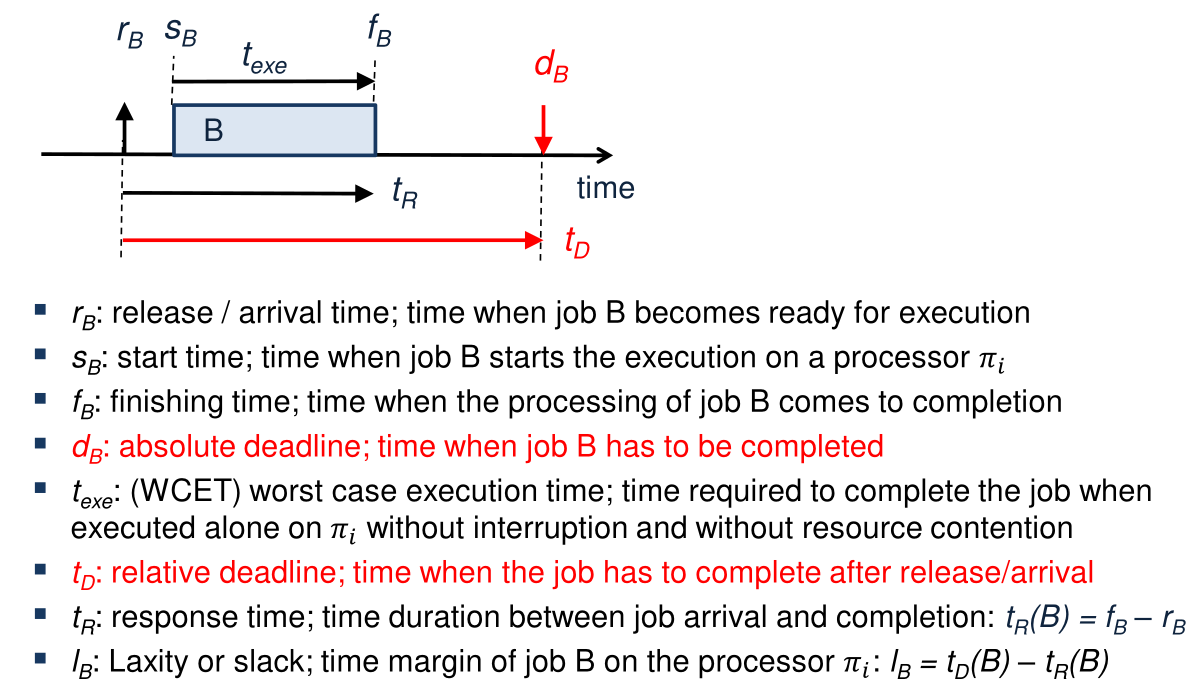
\includegraphics[width=\linewidth]{assets/RealTimeParameters.png}
  \label{fig:realtimeparameters}
\end{center}

\begin{center}
  \centering
  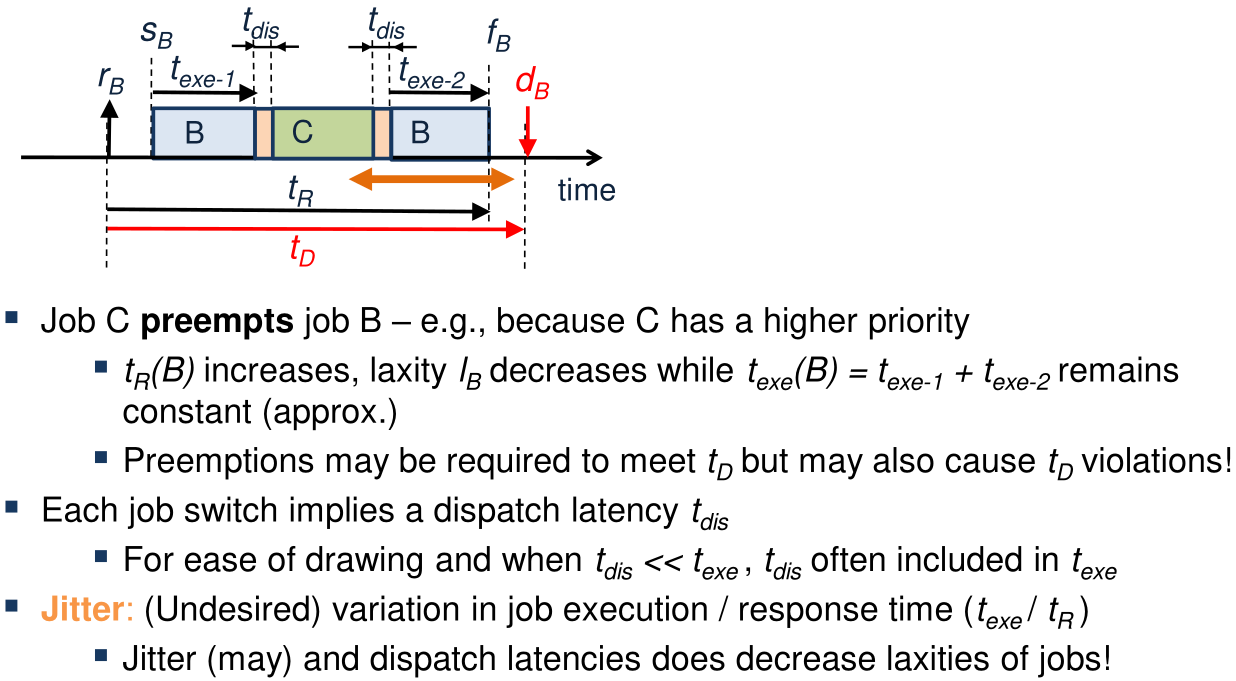
\includegraphics[width=\linewidth]{assets/RealTimeParameters2.png}
  \label{fig:realtimeparameters2}
\end{center}

\begin{center}
  \centering
  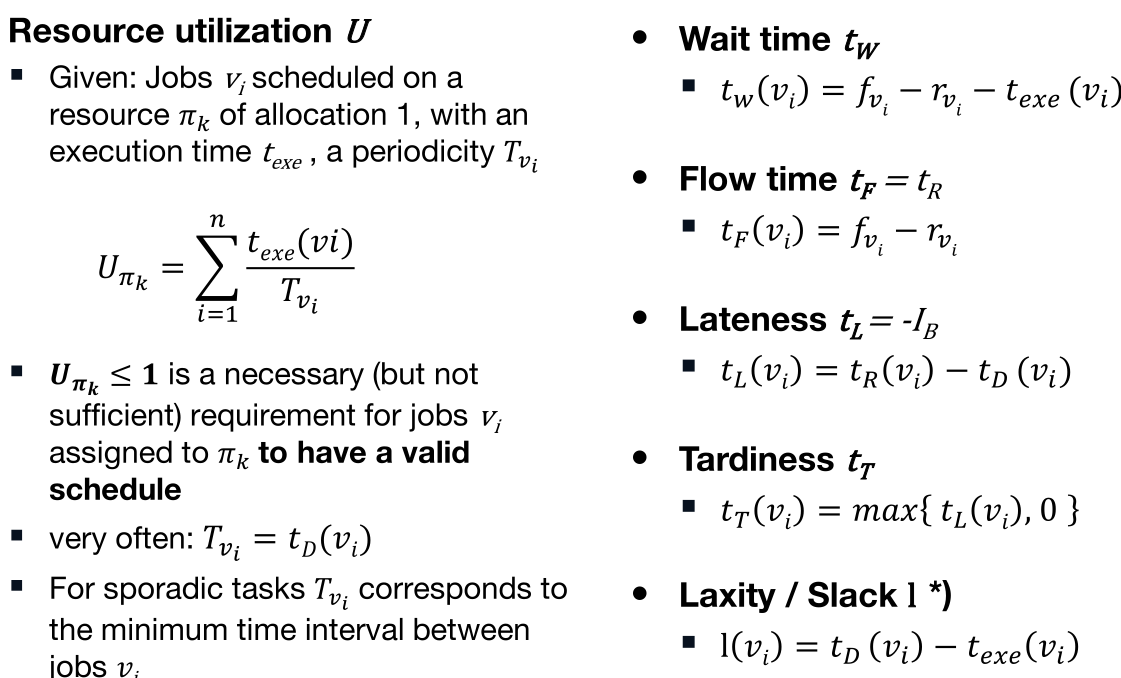
\includegraphics[width=\linewidth]{assets/SchedulingTimingMetrics.png}
  \label{fig:schedulingtimingmetrics}
\end{center}

\paragraph{Optimization Targets}

\begin{center}
  \centering
  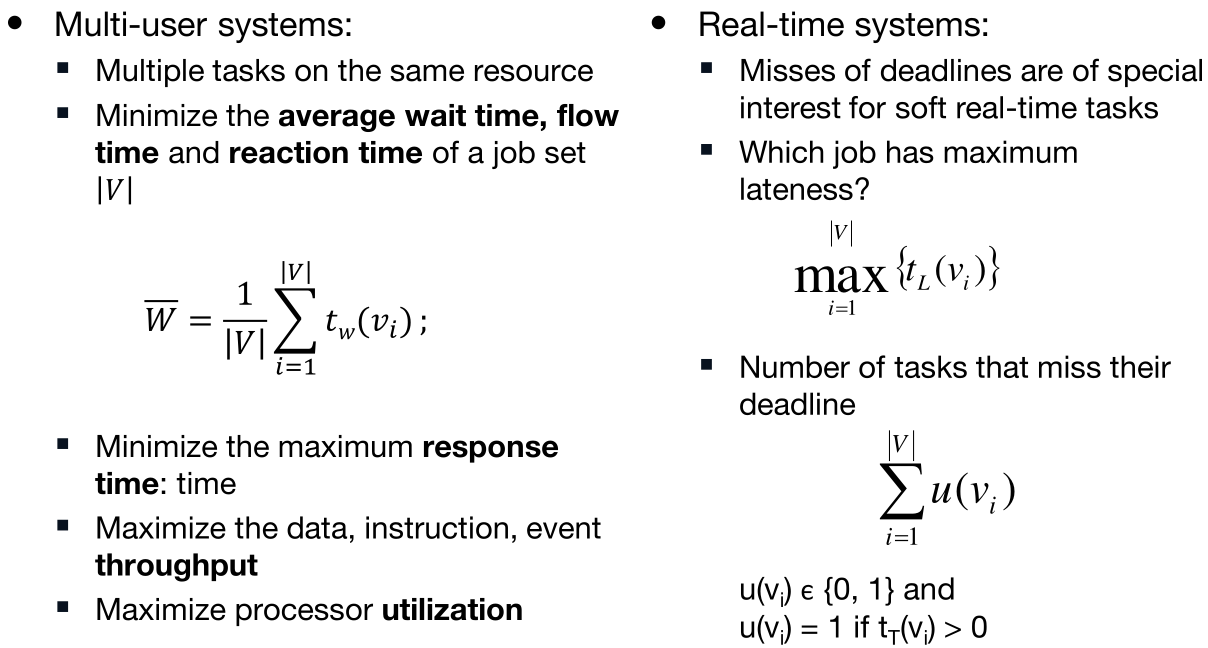
\includegraphics[width=\linewidth]{assets/OptimizationTargets.png}
  \label{fig:optimizationtargets}
\end{center}


\subsection{Dynamic Scheduling}

\textbf{preemptive}: Ability to preempt jobs or assign jobs after preemption to different processor resources creates “degrees of freedom” to achieve a feasible or improved schedule

\paragraph{Round robin (RR)}

\begin{center}
  \centering
  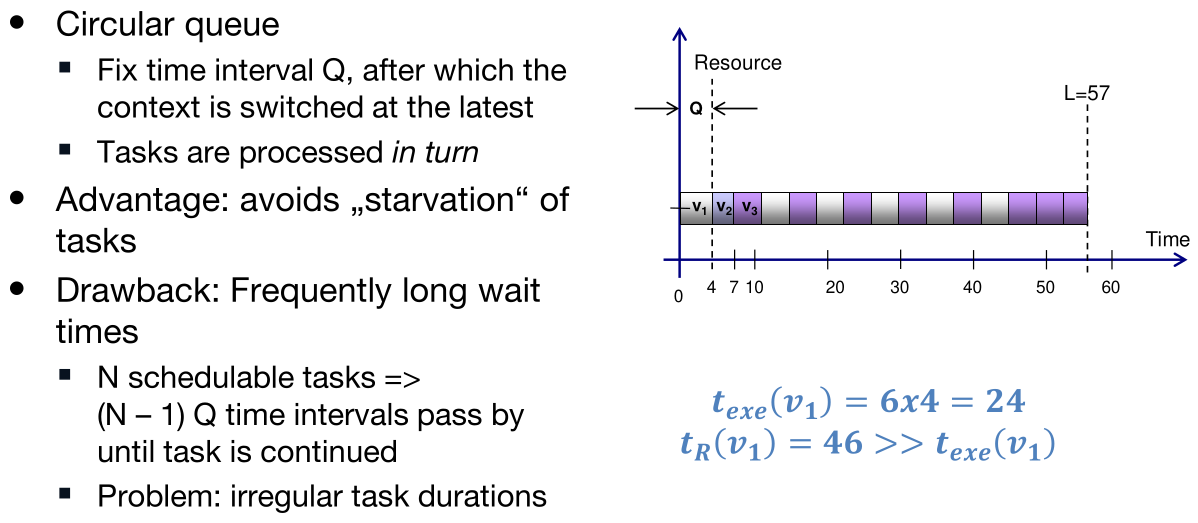
\includegraphics[width=\linewidth]{assets/RoundRobin.png}
  \label{fig:roundrobin}
\end{center}


\paragraph{First come first served}
\begin{center}
  \centering
  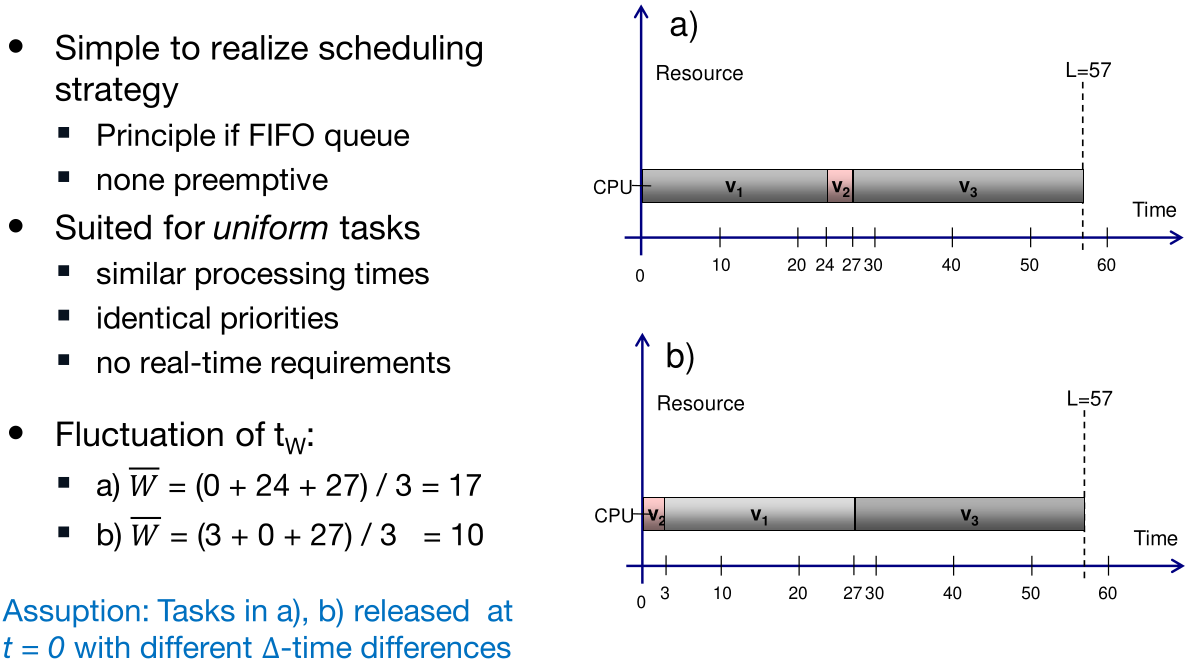
\includegraphics[width=\linewidth]{assets/FistComeFirstServed.png}
  \label{fig:fistcomefirstserved}
\end{center}
 
\paragraph{Shortest job first (SJF)}

\paragraph{Rate Monotonic Scheduling (RMS)}

\begin{center}
  \centering
  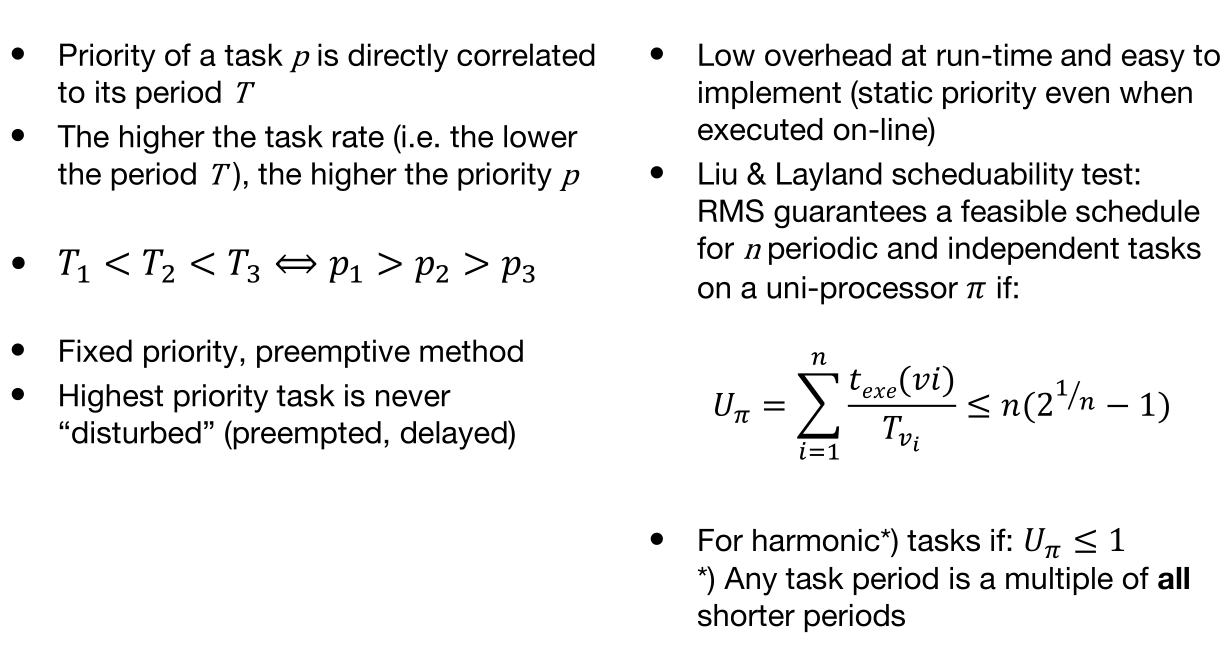
\includegraphics[width=\linewidth]{assets/RateMonotonicScheduling.png}
  \label{fig:ratemonotonicscheduling}
\end{center}

\textbf{Hyper Period} $H = lcm_i(T_i)$

\paragraph{Earliest Deadline First}

\paragraph{Shortest remaining time next (SRTN)}
preemptive

\paragraph{Least Laxity (LL)}

\paragraph{As soon as possible (ASAP)}
No resource constrains!

\paragraph{As Late As Possible (ALAP)}
\textbf{mobility}: Indicates a start time window of a job to still satisfy $t_D^L$ 

Jobs $v_i$ with lowest mobility $\mu$ are in critical path(s) of G(V, E)

$\mu(v_i) = s_{v_i}^{ALAP} - s_{v_i}^{ASAP}$

\paragraph{ASAP/ALAP with Conditional Task Shift}
Starting point is an ASAP/ALAP schedule

Check if schedule obeys resource constrain $\alpha(cpu) = 2; \alpha(acc) = 2$ 

In case of resource constraint violation, tasks with positive mobility are shifted to later(ASAP) / earlier (ALAP time slot)

\paragraph{List Scheduling} 


\begin{center}
  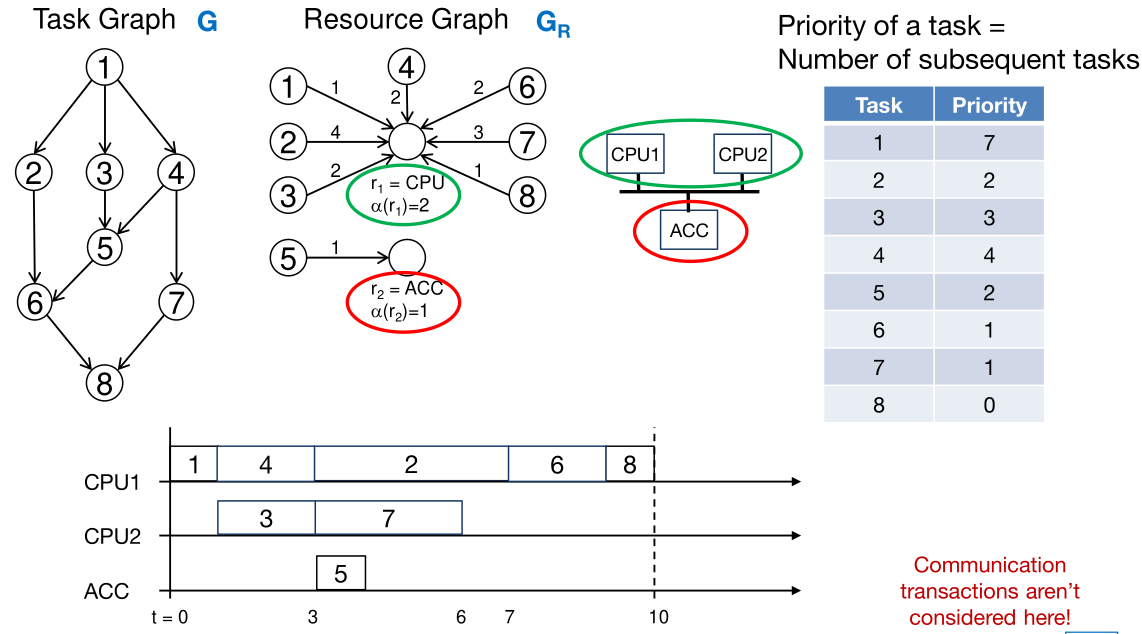
\includegraphics[width=0.8\linewidth]{assets/ListSchedulingExample.png}
  \label{fig:listschedulingexample}
\end{center}

\begin{center}
  \centering
  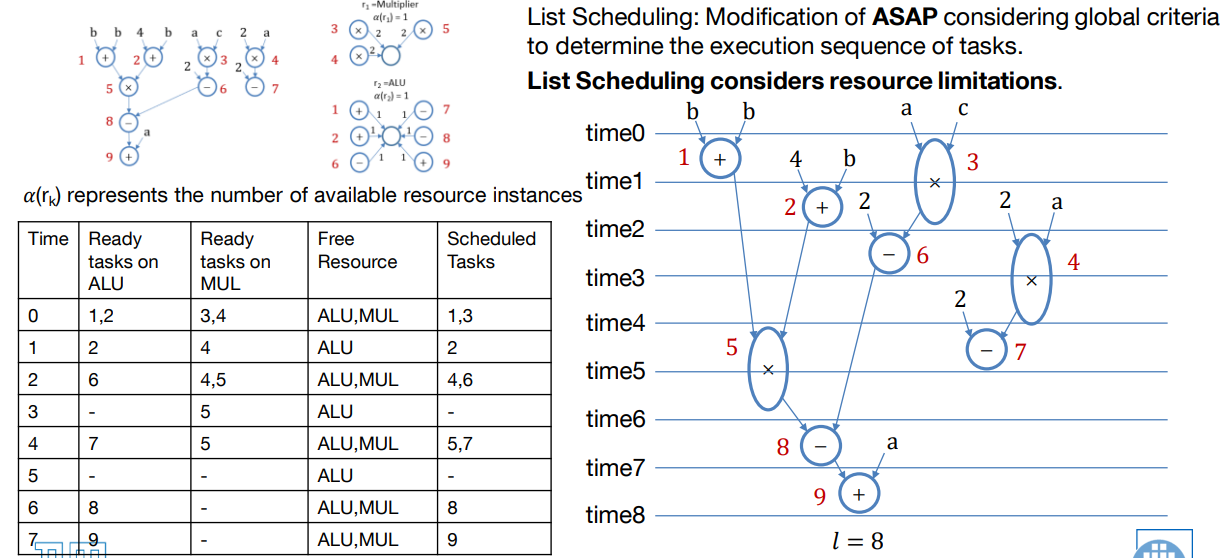
\includegraphics[width=0.8\linewidth]{assets/ListSchedulingTut.png}
  \label{fig:listschedulingtut}
\end{center}

\section{Design Estimation Techniques}

\textbf{Motivation}: Design parameter estimation allows to bound
relevant system aspects prior to system implementation

\paragraph{Estimation Metrics}

\begin{center}
  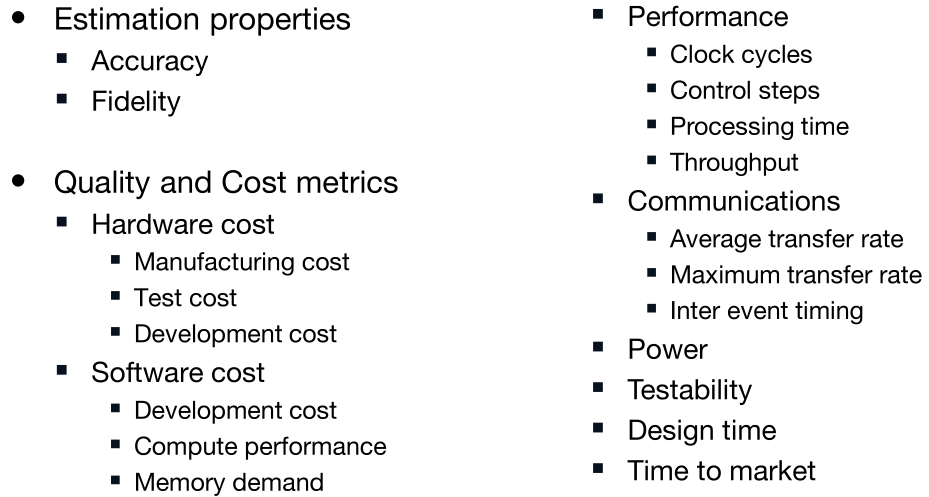
\includegraphics[width=0.8\linewidth]{assets/EstimationMetrics.png}
  \label{fig:estimationmetrics}
\end{center}

\paragraph{Trade off: Accuracy / Effort}


\paragraph{Accuracy / Fidelity - Definitions}
\begin{center}
  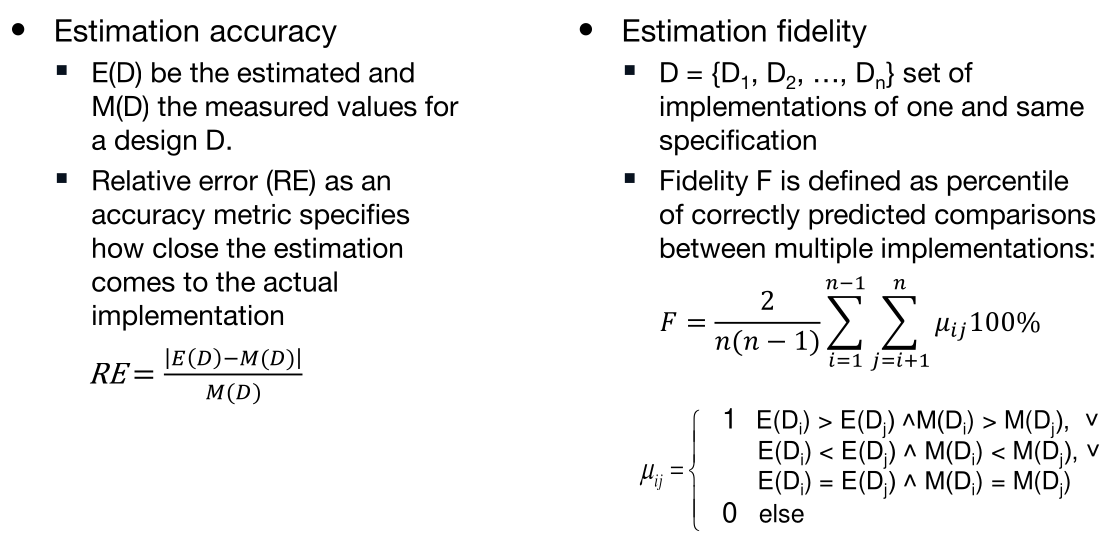
\includegraphics[width=\linewidth]{assets/AccuracyFidelityDefinitions.png}
  \label{fig:accuracyfidelitydefinitions}
\end{center}

For design space exploration choose fidelity over accuracy since the trend is more important than accurate measurement. If trend is corretct, ulitmately the best design point will be chosen anyway.

\paragraph{Hardware Cost Metrics}
\begin{enumerate}
	\item Manufacturing Cost
	\item Module Cost
	\item Test Cost
	\item Development Cost
\end{enumerate}

\paragraph{Hardware Performance Metrics}
Compute performance, Communication Bandwith
\begin{enumerate}
  \item Clock rate T
  \item Control Steps N
  \item Processing time/Latency $T_{ex} / L$
  \item Throughput R
\end{enumerate}
 
\paragraph{Software Cost Metrics}

\paragraph{Software Performance Metrics}
\begin{enumerate}
	\item MIPS (million instructions per second)
	\item Memory
	  \begin{enumerate}
	  	\item Access latency to different memory technologies in memory hierarchy
	  \end{enumerate}
\end{enumerate}

\paragraph{Communication Metrics}
\begin{enumerate}
	\item Maximum bit rate: PeakRate(C)
	\item Average bit rate: AvgRate(C)
\end{enumerate}

\paragraph{Other Metrics}
\begin{enumerate}
	\item Power dissipation
	\item Design-for-Test
	\item Development Time
	\item Time-to-market
\end{enumerate}

\paragraph{Hardware Estimation: FSMD Model}
Finite-State-Machine + Data Path

\paragraph{Clock Rate Estimation: Control Path}
$T_{clk} > \sum T_{logic} + T_{setup} + T_{pd}$
Logic depth (number of logic gates between registers) and wiring latencies determine FSM clock rate.

\paragraph{Maximum Operator Latency}
$T_{clk} = max_k(delay(r_k))$

\paragraph{Clock Rate Utilization: Slack}

\begin{center}
  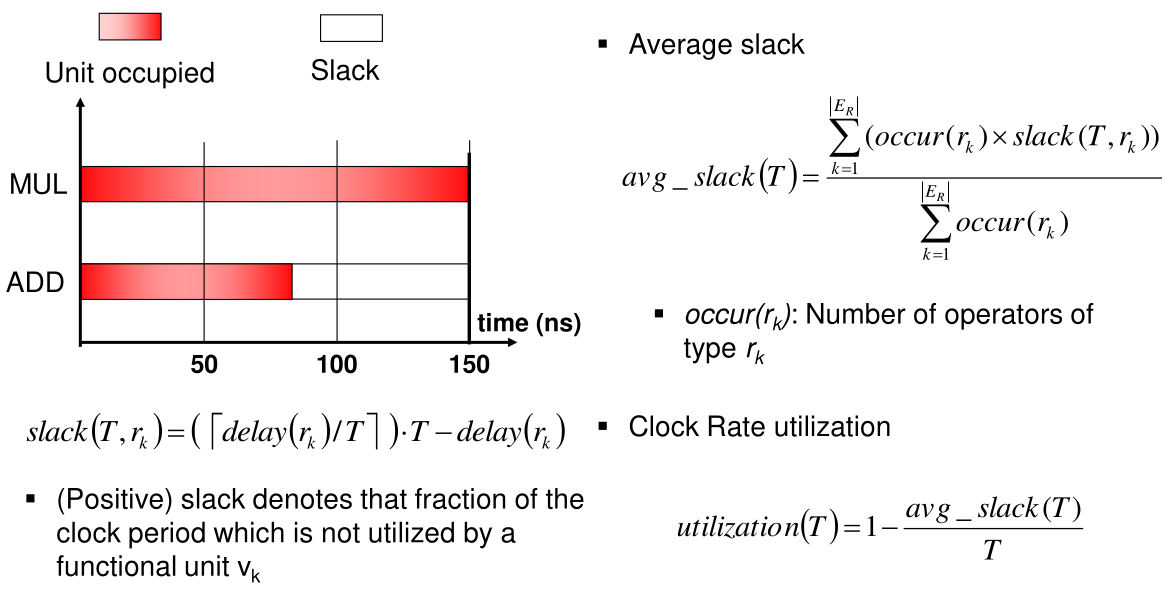
\includegraphics[width=\linewidth]{assets/Slack.png}
  \label{fig:slack}
\end{center}

\paragraph{Pipelining}

\paragraph{Generic Model}
Estimate independent of CPU Model.

\textbf{Worst Case Execution Time (WCET)}
Hard real time requirements have to be met.

\paragraph{Program Exeution Time $T_{ex}$}
$T_{ex} = \frac{Instructions}{Program} \frac{clockCycles}{Instructions} \frac{seconds}{clockCycle)}$

\paragraph{Instruction Count Estimation with DFG / CFG}

\begin{center}
  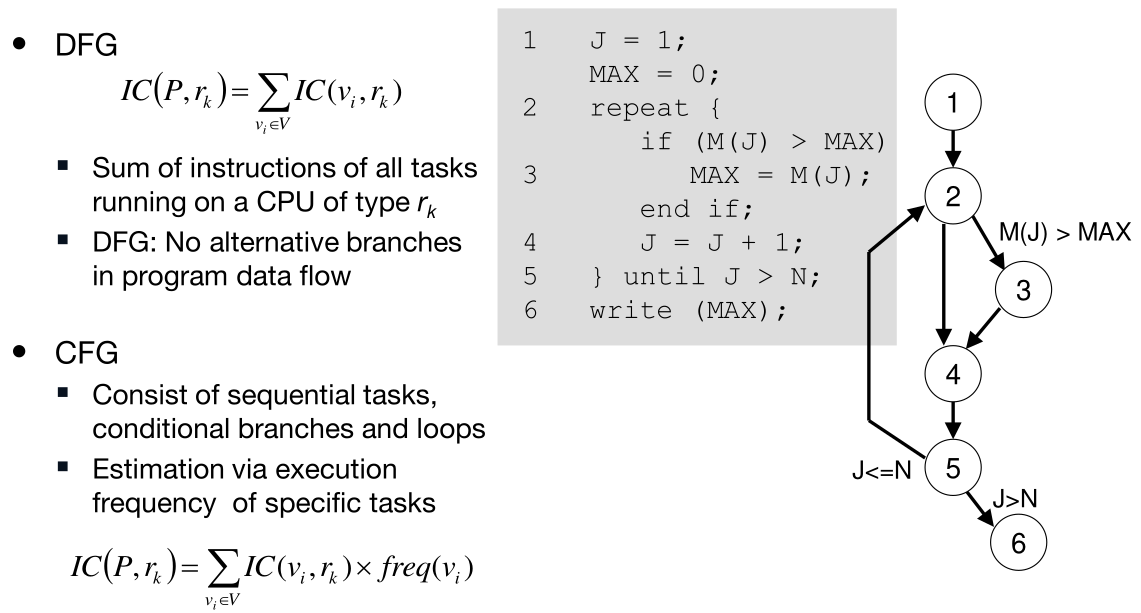
\includegraphics[width=\linewidth]{assets/InstructionCountEstDFG.png}
  \label{fig:instructioncountestdfg}
\end{center}


\begin{center}
  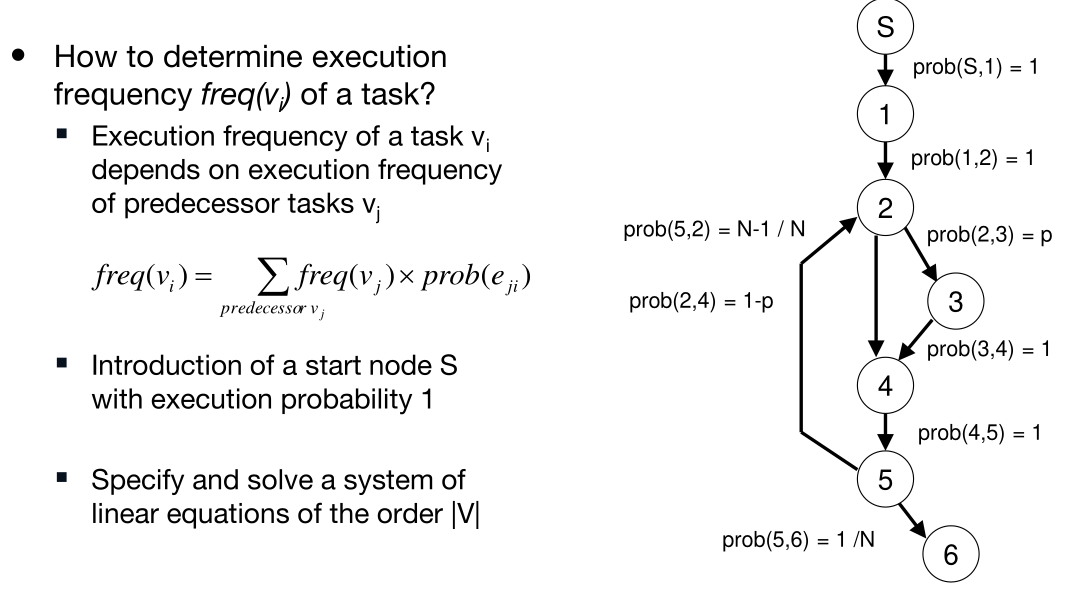
\includegraphics[width=\linewidth]{assets/ICECFG.png}
  \label{fig:icecfg}
\end{center}

% ======================================================================
% End
% ======================================================================
\end{document}
